\documentclass{article}

\usepackage[utf8]{inputenc}
\usepackage[T1]{fontenc}
\usepackage[spanish]{babel} % Cambia "spanish" por tu idioma si es diferente
\usepackage{graphicx}
\usepackage{hyperref}

\begin{document}

\tableofcontents 

\section{Introducción a Python}

\subsection{¿Qué es Python?}
Python es un lenguaje de programación, lo que este está diseñado para una fácil comprensión para los seres humanos. Fue creado por Guido van Rossum, lanzó su primera versión en 1991, Python ha ganado popularidad y se ha convertido en uno de los lenguajes de programación.\\

El diseño de Python se centra en la simplicidad y la elegancia lo que facilita a los desarrolladores escribir códigos claros y concisos.

Python es un lenguaje interpretado, lo que significa que el código escrito por los programadores se traduce a un lenguaje intermedio que luego es ejecutado por el intérprete de Python, esto permite un rápido desarrollo, ya que los programadores pueden ver el resultado de su código inmediatamente después de escribirlo.\\

Utiliza ``indentación'' para definir bloques de código, lo que elimina la necesidad de palabras claves adicionales, esto hace que el código sea limpio y fácil de leer.
Python es un lenguaje multiparadigma, lo que significa que está orientada a programación con objetos como programación estructurada, esto permite a los desarrolladores utilizar diferentes enfoques según las necesidades de su proyecto. Además Python tiene una gran biblioteca estándar que proporciona módulos y paquetes para diversas aplicaciones, desde desarrollo web hasta procesamiento de datos
y cálculos científicos 

\subsection{Ventajas de usar Python}
\begin{enumerate}
    \item Es un lenguaje de sintaxis amplia y legible: Al ser lenguaje de programación de alto nivel, diseñado para que los algoritmos sean expresados de forma clara y fácilmente entendibles por los seres humanos.
    \item Ampliamente utilizado en múltiples campos: Su amplia variedad de usos lo ha dejado como el primero en el top 10 de los lenguajes de programación más utilizados según Tiobe, extraídos de las habilidades más desarrolladas por desarrolladores, empresas del sector y terceros.
    \item Python posee una gran cantidad de bibliotecas y frameworks : La gran cantidad de usos de Python se traduce en múltiples librerías y frameworks que ayudan a llevar a cabo funcionalidades. En sí mismo ya tiene una biblioteca estándar y podemos encontrar hasta 135. 000+ más para diversas aplicaciones. Sin embargo, entre las más populares según el sitio de AWS se encuentran Matplotlib, Pandas, Request, Numpy, Keras y OpenCV-Python. Esta variedad no se limita solo a las librerías. Así mismo la podemos encontrar en los marcos o frameworks, que facilitan el proceso de creación debido a que ahorra el proceso de escritura de un código. 
    \item Fácil portabilidad: Python es uno de los lenguajes de programación más portátiles y versátiles disponibles. Debido a que es un lenguaje de programación interpretado, en lugar de un lenguaje compilado, se puede ejecutar en una amplia variedad de sistemas operativos y plataformas de hardware sin necesidad de realizar ajustes o cambios significativos en el código fuente.
    \item Tiene una gran comunidad de desarrolladores : Es una herramienta que constantemente evoluciona para suplir las necesidades que poco a poco van surgiendo en el campo de la tecnología, como hemos visto hasta ahora en sus usos para el machine learning.
    \item Multiplataforma: Python es uno de esos lenguajes de programación que puede ser ejecutado en cualquier sistema operativo en el cual se opere. Así es: no importa si se trata de Windows, Linux, macOS, y otros, este se puede ejecutar sin problema. Y, lo mejor, es que se desarrolla el código una única vez y podrá emplearse en los demás SO. 
\end{enumerate}

\section{Instalación y configuración del entorno de desarrollo}

\subsection{Descarga e instalación de Python}
A continuación, te dejaré un video para aprender de manera más práctica y visual, tienes que seguir los pasos que se mencionan: \href{https://www.youtube.com/watch?v=cmItObuFBuA}{Tutorial}

\begin{figure}[h]
    \centering
    \scalebox{0.35}{
    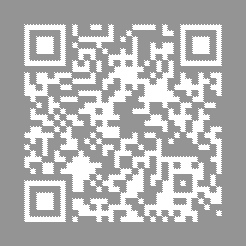
\includegraphics{Imagenes/instalacion1.png}
    }
  \end{figure}

Siguiendo con algo más teórico, para comenzar a programar en Python, primero necesitas instalar Python en tu sistema. Puedes hacerlo siguiendo estos pasos:

\begin{itemize}
    \item[a. ]Descarga Python: Visita el sitio web oficial de Python en python.org y descarga la última versión de Python. Asegúrate de elegir la versión más reciente y compatible con tu sistema operativo (Windows, macOS, o Linux).
    \begin{figure}[h]
        \centering
        \scalebox{0.35}{
        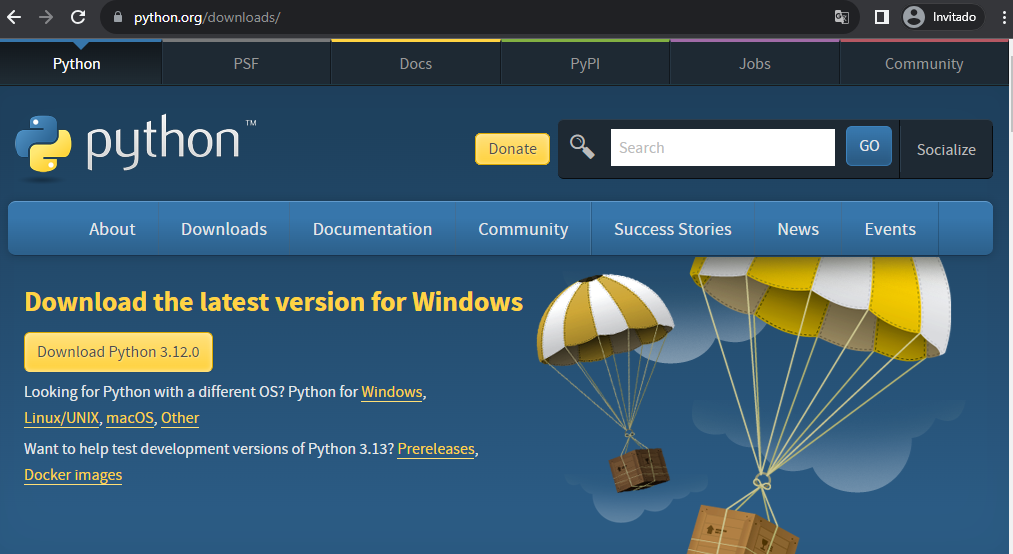
\includegraphics{Imagenes/instalacion2.png}
        }
      \end{figure}
    
    \item[b. ]Instalación en Windows: Ejecuta el archivo descargado y sigue las instrucciones del instalador. Asegúrate de marcar la opción ``Agregar Python al PATH'' durante la instalación.
    \begin{figure}[h]
        \centering
        \scalebox{0.35}{
        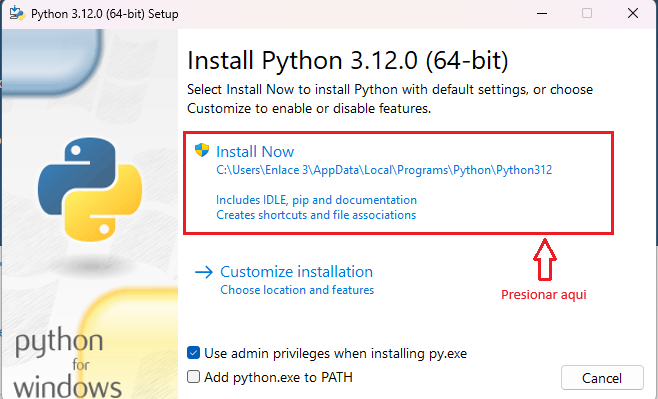
\includegraphics{Imagenes/instalacion3.png}
        }
      \end{figure}
\end{itemize}

\subsection{Configuración del entorno de desarrollo}
Puedes escribir y ejecutar código Python en un entorno de desarrollo integrado (IDE) o simplemente en un editor de texto. Algunas opciones populares para IDEs incluyen:\\

Elige el IDE o editor de tu preferencia y configúralo.
\begin{itemize}
    \item IDLE: es un programa que te ayuda a escribir y ejecutar código en Python. Es útil para principiantes porque combina un espacio para escribir código y un lugar para ver los resultados, lo que facilita aprender y probar cosas nuevas en Python. Tutorial de Cómo instalar Python y usar la herramienta IDLE: 
    \href{https://www.youtube.com/watch?v=F9eM_VoKGJQ}{Revisa este link para más ayuda}
    \begin{figure}[h]
        \centering
        \scalebox{0.35}{
        
\includegraphics{Imagenes/instalacion4.png}
        }
      \end{figure}

    \item PyCharm: Un IDE muy popular y potente para Python. Tutorial de Como instalar y configurar Pycharm:
    \href{https://www.youtube.com/watch?v=wxdafAAzIWo }{Revisa este link para más ayuda}
    \begin{figure}[h]
        \centering
        \scalebox{0.35}{
        
\includegraphics{Imagenes/instalacion5.png}
        }
      \end{figure}

    \item Visual Studio Code (VSCode): Un editor de código que es altamente configurable y ampliamente utilizado para Python. Tutorial de como instalar y Configurar Visual Studio Code:
    \href{https://www.youtube.com/watch?v=X_Z7d04x9-E}{Revisa este link para más ayuda}
    \begin{figure}[h]
        \centering
        \scalebox{0.35}{
        
\includegraphics{Imagenes/instalacion6.png}
        }
      \end{figure}
\end{itemize}

\subsection{Tu primer programa en python}

Una vez que hayas instalado Python y configurado tu entorno de desarrollo, puedes comenzar a escribir código Python. Aquí tienes un ejemplo de un programa Python simple:
\begin{figure}[h]
    \centering
    \scalebox{0.35}{
    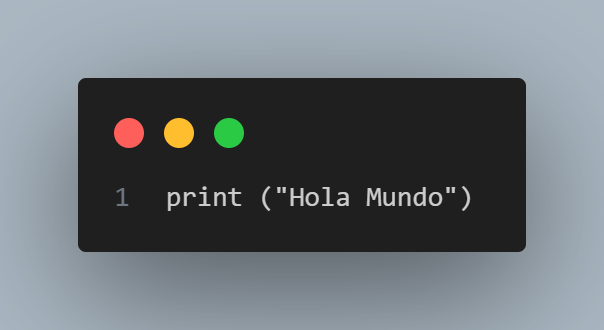
\includegraphics{Imagenes/instalacion7.png}
    }
  \end{figure}
Para ejecutar el código, guárdalo en un archivo con extensión ``.py'' (por ejemplo, ``mi\_programa.py'') y ejecútalo desde la línea de comandos o desde tu IDE.



\section{Fundamentos de la sintaxis de Python}

Python se destaca por su legibilidad y simplicidad. Algunas pautas importantes de la sintaxis incluyen:

\subsection{Variables y asignaciones}
Las variables en Python son contenedores que se utilizan para almacenar datos. Estos datos pueden ser números, cadenas de texto, listas, objetos o cualquier otro tipo de información que necesites en tu programa. Las variables te permiten acceder, modificar y manipular datos de manera dinámica en tu código.\\

Declaración y Asignación: Para crear una variable en Python, simplemente elige un nombre descriptivo y utiliza el operador de asignación ``$=$'' para darle un valor. La estructura general es la siguiente:

\begin{figure}[h]
    \centering
    \scalebox{0.35}{
    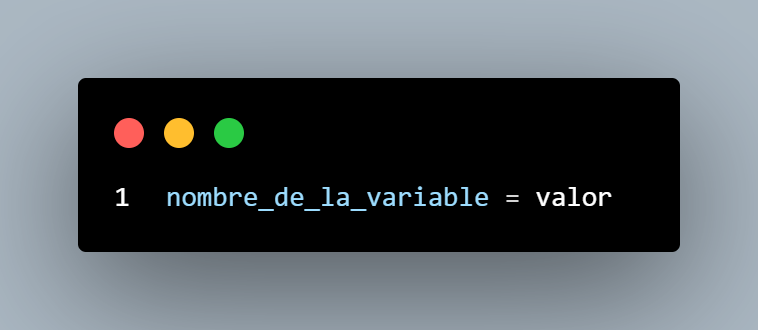
\includegraphics{Imagenes/funadamentos1.png}
    }
  \end{figure}

\begin{itemize}
    \item ``nombre\_de\_la\_variable'': Es el nombre que eliges para la variable. Debe seguir las reglas de nomenclatura y convenciones de nombres que se mencionaron previamente.  
    \item ``valor'': Es el dato que deseas almacenar en la variable. Puede ser un número, una cadena de texto, un resultado de cálculos, una lista, un objeto, etc.
\end{itemize}

\begin{figure}[h]
    \centering
    \scalebox{0.35}{
    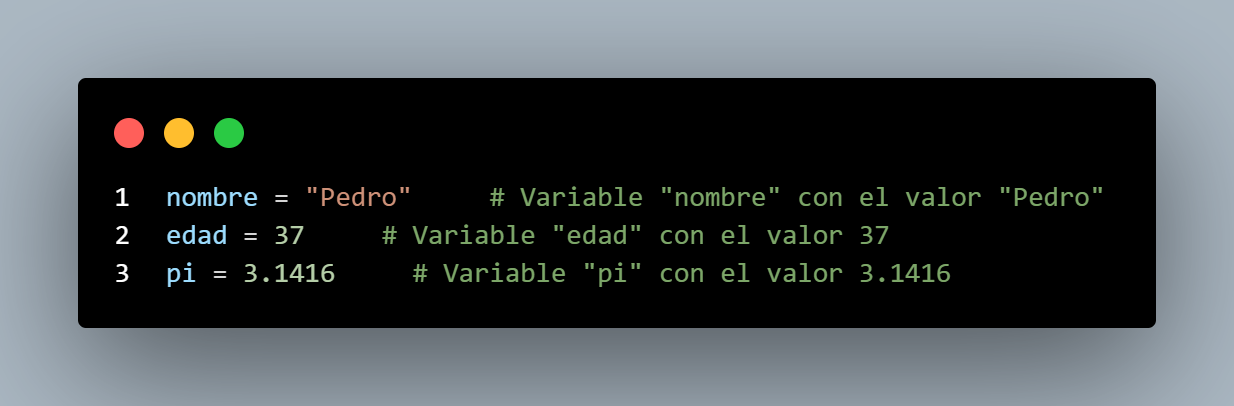
\includegraphics{Imagenes/fundamentos2.png}
    }
  \end{figure}

Reasignación de variables: Puedes cambiar el valor de una variable en cualquier momento asignándole un nuevo valor:\\
\begin{figure}[h]
    \centering
    \scalebox{0.35}{
    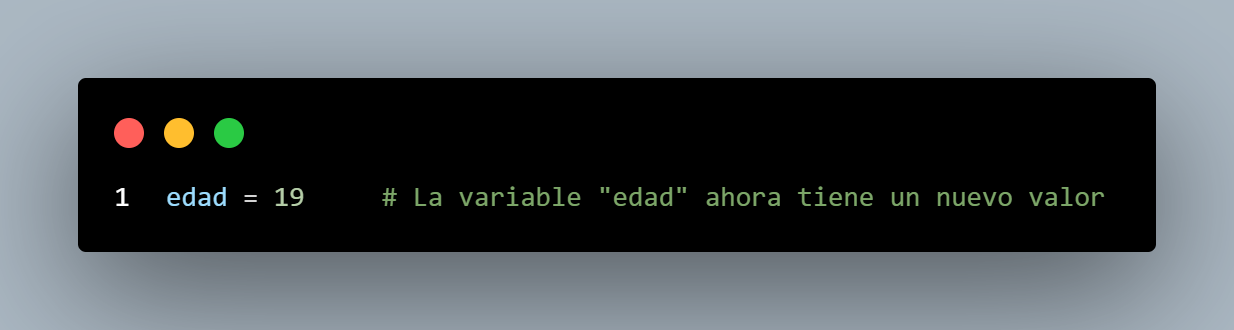
\includegraphics{Imagenes/fundamentos3.png}
    }
  \end{figure}

Identificadores: Los identificadores son nombres que se utilizan para representar variables, funciones, clases y otros elementos en Python. Algunas reglas claves para los identificadores en Python son:

\begin{itemize}
    \item Deben comenzar con una letra (mayúscula o minúscula) o un guión bajo ``\_''.
    \item Pueden contener letras, números y guiones bajos.
    \item Python distingue entre mayúsculas y minúsculas, por lo que mi\_variable y Mi\_Variable son consideradas diferentes.
    \item No se pueden utilizar palabras clave de Python como identificadores. Las palabras clave son términos reservados para funciones y estructuras de control, como ``if'', ``for'', ``while'', entre otros.
\end{itemize}

\begin{figure}[h]
    \centering
    \scalebox{0.35}{
    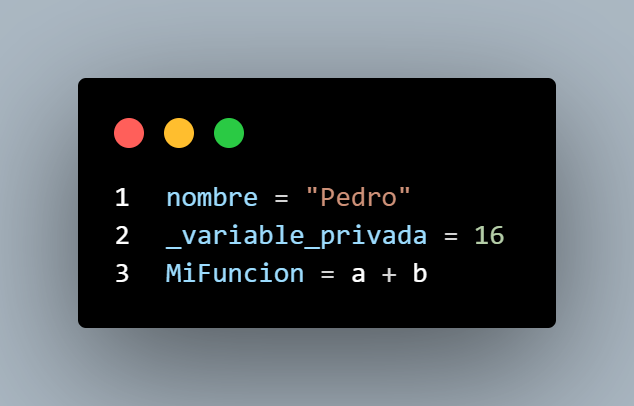
\includegraphics{Imagenes/fundamentos4.png}
    }
  \end{figure}

Uso de variables: Las variables se utilizan para almacenar valores y realizar cálculos. Puedes utilizar variables en expresiones matemáticas, en operaciones de cadena de texto, en estructuras de control (como condicionales y bucles) y para muchas otras tareas en tu programa.\\

\begin{figure}[h]
    \centering
    \scalebox{0.35}{
    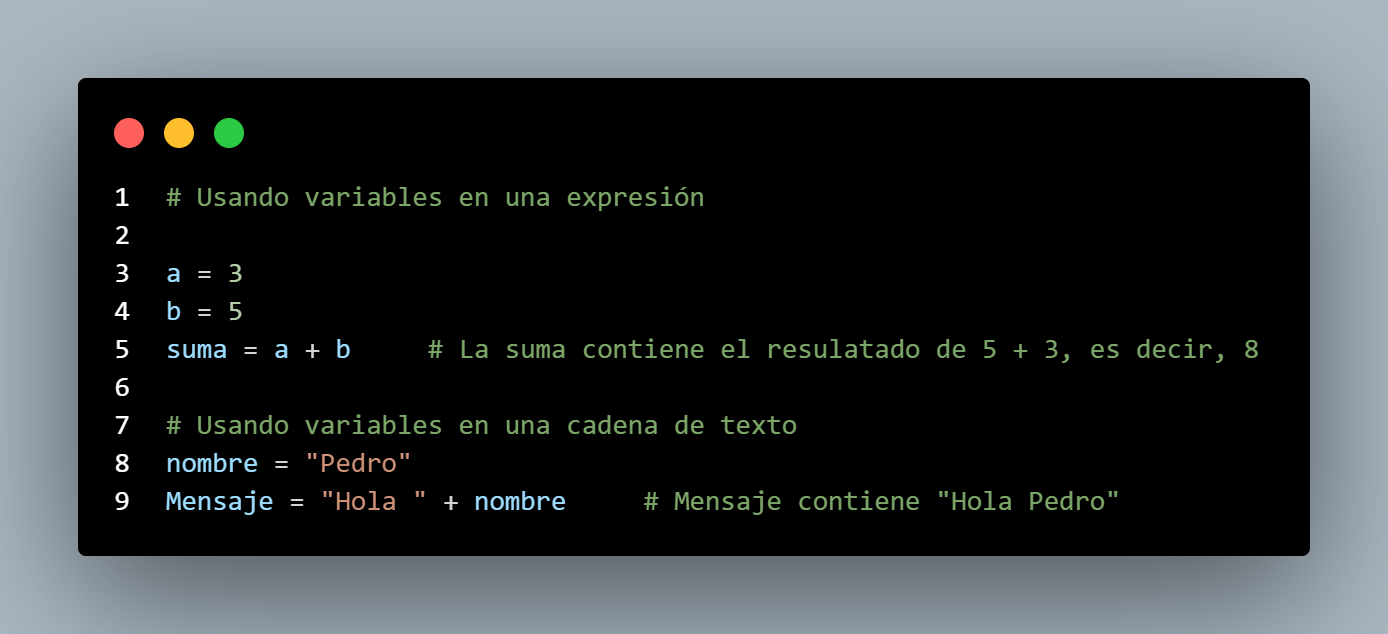
\includegraphics{Imagenes/fundamentos5.png}
    }
  \end{figure}

Constantes: Puedes usar variables para definir constantes, que son valores que no deben modificarse a lo largo del programa. Para indicar que una variable es una constante, es común utilizar letras mayúsculas y subrayados (por ejemplo, PI = 3.1416).\\

Desestructuración de Asignación: Python permite asignar valores a Múltiples variables en una sola línea de código. Esto es especialmente útil cuando se trabaja con secuencias como listas o tuplas.

\begin{figure}[h]
    \centering
    \scalebox{0.35}{
    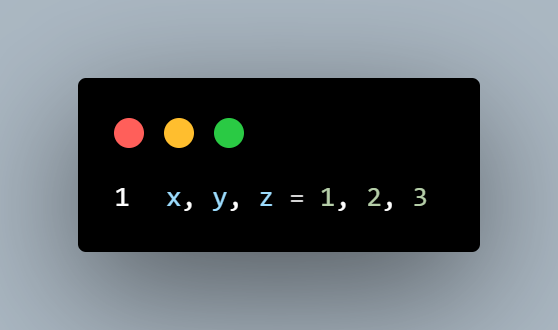
\includegraphics{Imagenes/fundamentos6.png}
    }
  \end{figure}

Operadores de Asignación Combinada: Python ofrece operadores de asignación combinada que permiten simplificar la asignación de variables en operaciones comunes. Por ejemplo, ``+='' es una forma abreviada de incrementar el valor de una variable.\\

\begin{figure}[h]
    \centering
    \scalebox{0.35}{
    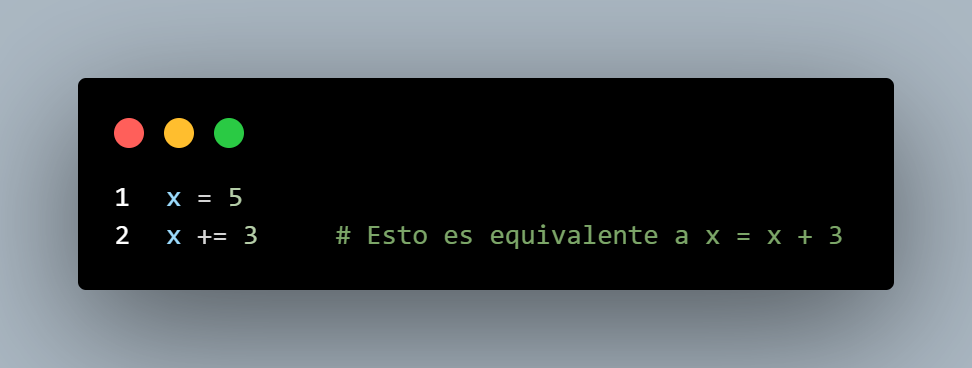
\includegraphics{Imagenes/fundamentos7.png}
    }
  \end{figure}

Tipos de datos: Python es un lenguaje de tipo dinámico, lo que significa que una variable no tiene un tipo de dato fijo. El tipo de dato de una variable se asigna automáticamente según el valor que contiene. Puedes verificar el tipo de dato de una variable utilizando la función ``type()'':\newpage

\begin{figure}[h]
    \centering
    \scalebox{0.35}{
    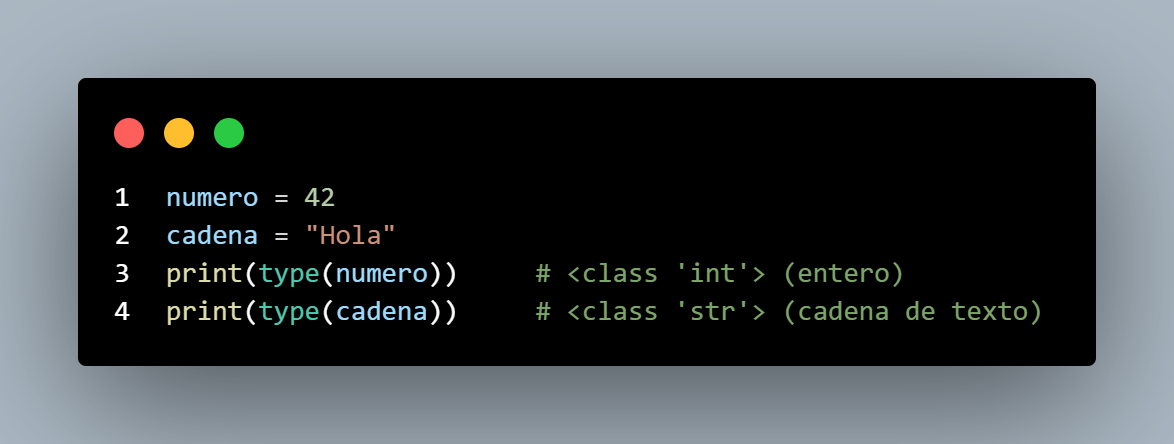
\includegraphics{Imagenes/fundamentos8.png}
    }
  \end{figure}

Ámbito de variables: Las variables pueden tener un ámbito local o global:

\begin{itemize}
    \item Ámbito local: Las variables declaradas dentro de una función tienen un ámbito local y solo son accesibles dentro de esa función.
\end{itemize}

    \begin{figure}[h]
        \centering
        \scalebox{0.35}{
        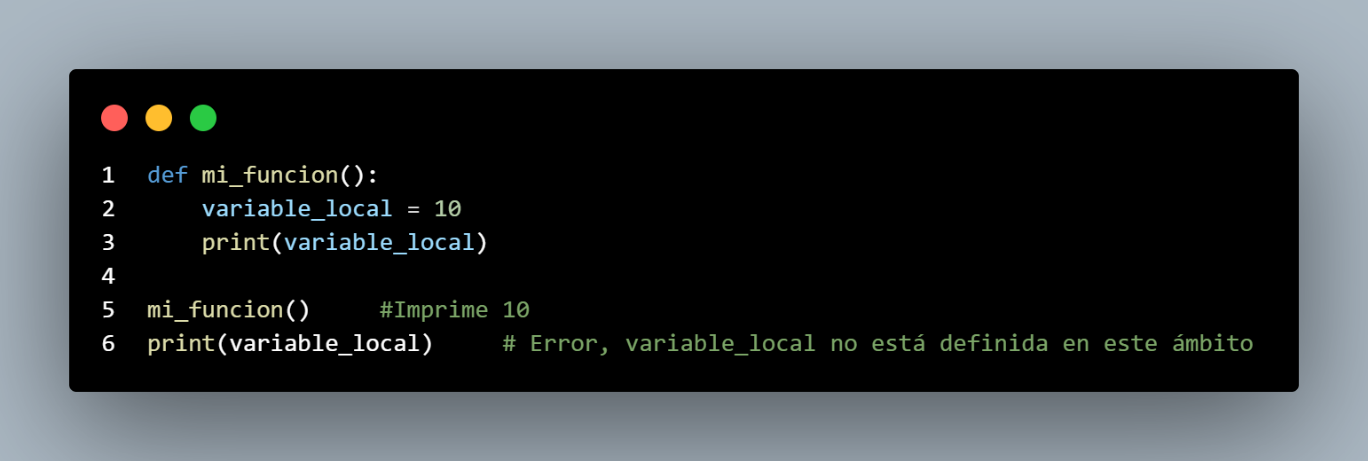
\includegraphics{Imagenes/fundamentos9.png}
        }
      \end{figure}


\begin{itemize}
    \item Ámbito Global: Las variables declaradas fuera de una función o declaradas como globales dentro de una función tienen un ámbito global y son accesibles desde cualquier parte del código.
\end{itemize}

    \begin{figure}[h]
        \centering
        \scalebox{0.33}{
        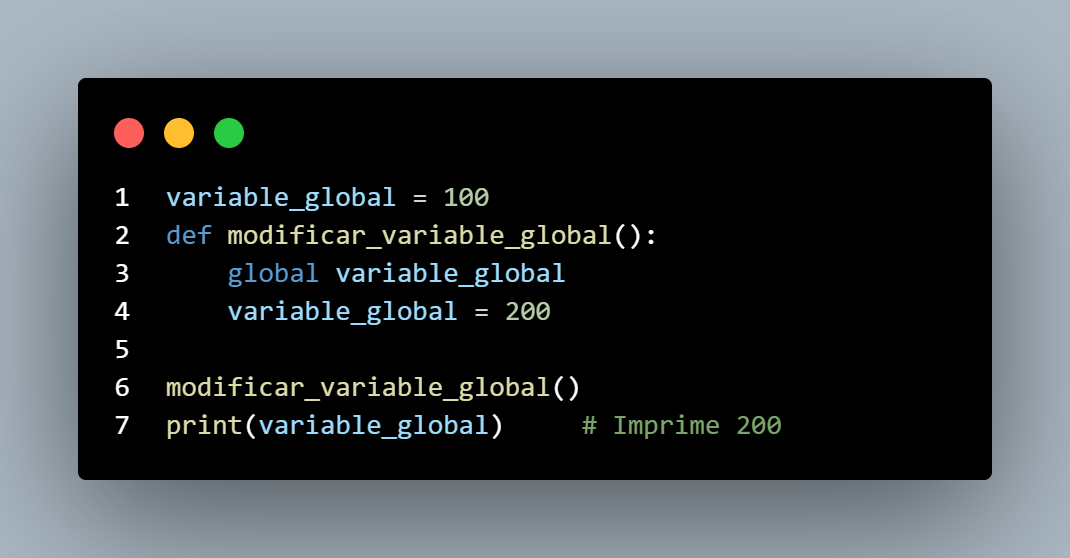
\includegraphics{Imagenes/fundamentos10.png}
        }
      \end{figure}
\newpage

Ejemplo usando ambos:

\begin{figure}[h]
    \centering
    \scalebox{0.35}{
    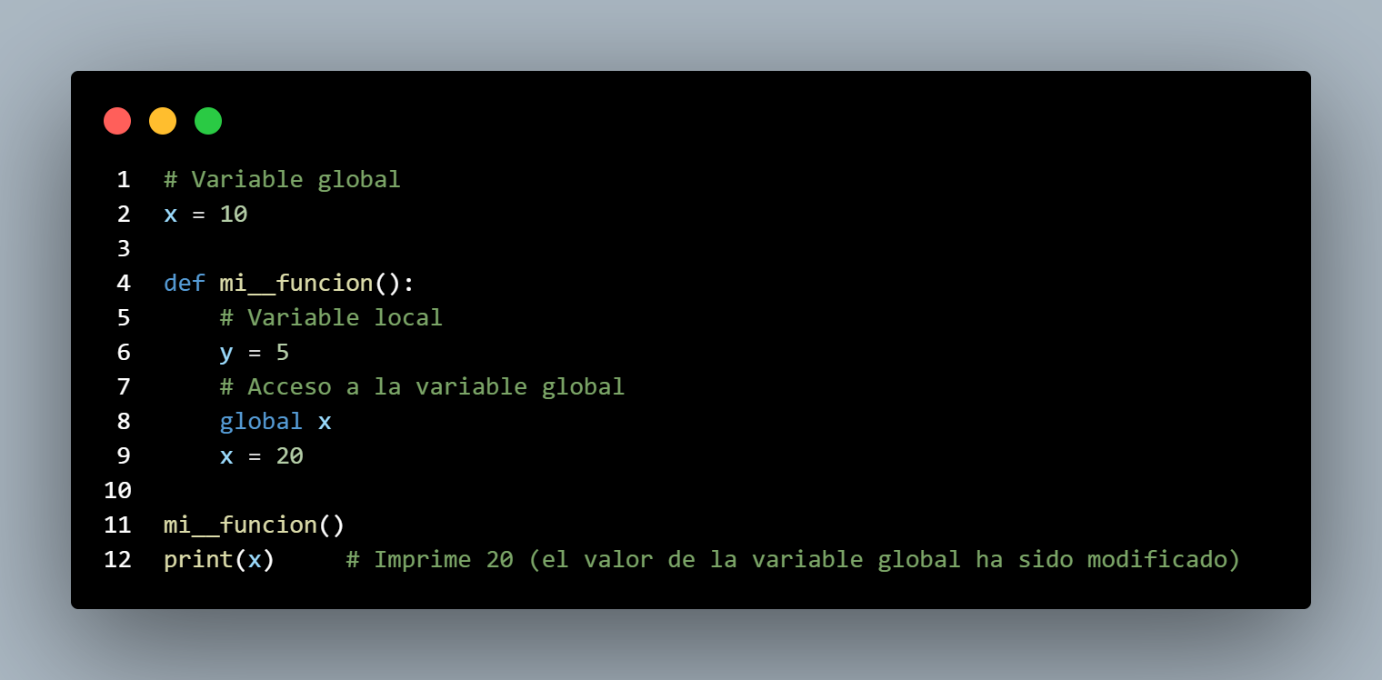
\includegraphics{Imagenes/fundamentos11.png}
    }
  \end{figure}

Estos son algunos aspectos adicionales relacionados con las variables en Python que pueden ser útiles para comprender en tu proceso de aprendizaje.

\subsection{Operadores Aritmeticos}
Los operadores aritméticos en Python se utilizan para realizar operaciones matemáticas. 

Los principales son:
\begin{itemize}
    \item Suma (+): Se utiliza para sumar dos valores.
    \item Resta (-): Se utiliza para restar un valor de otro.
    \item Multiplicación (*): Se utiliza para multiplicar dos valores.
    \item División (/): Se utiliza para dividir un valor por otro.
    \item División Entera (//): Devuelve la parte entera de la división entre dos valores.
    \item Módulo (\%): Devuelve el resto de la división entre dos valores.
    \item Potencia (**): Eleva un valor a una potencia.
  \end{itemize}  

\subsection{Operadores de comparación}
Los operadores de comparación se utilizan para comparar dos valores y devuelven un valor booleano (True o False). 

Los principales son:
\begin{itemize}
    \item Igual (==): Comprueba si dos valores son iguales.
    \item No Igual (!=): Comprueba si dos valores no son iguales.
    \item Mayor que (>): Comprueba si un valor es mayor que otro. En caso de strings se compara cadenas de caracteres lexicográficamente (es decir, en función del orden alfabético).
    \item Menor que (<): Comprueba si un valor es menor que otro.En caso de strings se compara cadenas de caracteres lexicográficamente (es decir, en función del orden alfabético).
    \item Mayor o igual que (>=): Comprueba si un valor es mayor o igual que otro.En caso de strings se compara cadenas de caracteres lexicográficamente (es decir, en función del orden alfabético).
    \item Menor o igual que (<=): Comprueba si un valor es menor o igual que otro. En caso de strings se compara cadenas de caracteres lexicográficamente (es decir, en función del orden alfabético).
\end{itemize}

\subsection{Operadores lógicos}
Los operadores lógicos se utilizan para combinar expresiones lógicas y devuelven un valor booleano. 

Los principales son:
\begin{itemize}
    \item and: Devuelve True si ambas expresiones son True.
    \item or: Devuelve True si al menos una de las expresiones es True.
    \item not: Devuelve el inverso de la expresión.
\end{itemize}

\subsection{Operadores de asignación}
Los operadores de asignación se utilizan para asignar valores a variables. Algunos de ellos incluyen:
\begin{itemize}
    \item =: Asigna un valor a una variable.
    \item +=: Suma y asigna el resultado a la variable.
    \item -=: Resta y asigna el resultado a la variable.
    \item *=: Multiplica y asigna el resultado a la variable.
    \item /=: Divide y asigna el resultado a la variable.
\end{itemize}

\subsection{Operadores de pertenencia e identidad}
\begin{itemize}
    \item Operadores de Pertenencia: `in` y `not in` se utilizan para verificar si un elemento está presente en una secuencia (como una lista, tupla, etc.)
    \item Operadores de Identidad: `is` y `is not` se utilizan para verificar si dos objetos tienen la misma identidad (es decir, si son el mismo objeto en la memoria).
\end{itemize}

\subsection{Expresiones}
Una expresión es una combinación de valores, variables y operadores que se evalúa para producir un resultado. Las expresiones se utilizan en muchas partes del código, como asignaciones, condicionales, bucles y funciones. Por ejemplo:\\

\begin{figure}[h]
    \centering
    \scalebox{0.35}{
    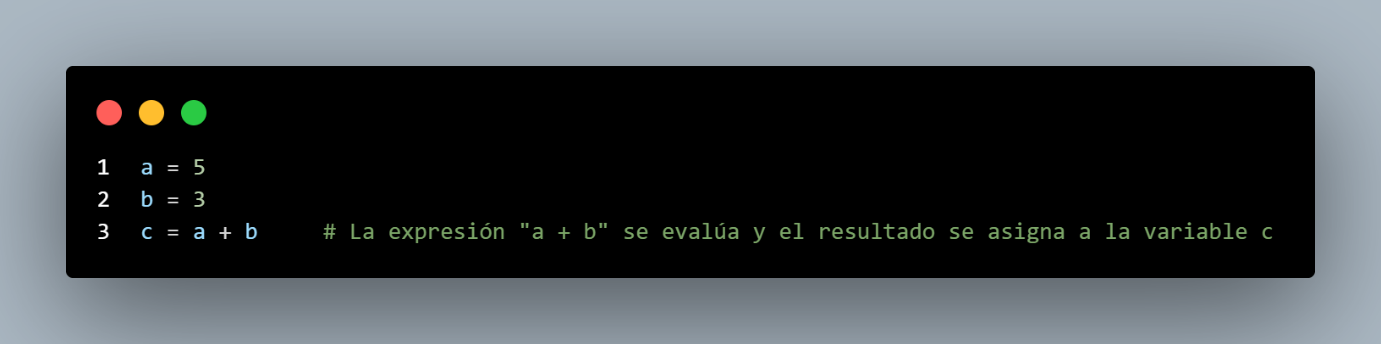
\includegraphics{Imagenes/fundamentos12.png}
    }
  \end{figure}
Las expresiones pueden ser tan simples como una sola variable o tan complejas como cálculos matemáticos o lógicos.

Estos son los operadores y las expresiones en Python que son fundamentales para realizar tareas de cálculo, toma de decisiones y procesamiento de datos en tus programas. Puedes combinar estos operadores y expresiones de diversas maneras para realizar tareas específicas en tu código.

\subsection{Comentarios y formato de código}
Los comentarios y el formato de código son aspectos cruciales de la programación en Python. Los comentarios son notas en el código que se utilizan para explicar lo que hace el código, mientras que el formato se refiere a la estructura y el estilo del código para que sea más legible y mantenible.\\

Comentarios: Los comentarios en Python se utilizan para agregar explicaciones o notas al código fuente. Se inician con el símbolo ``\#'' y Python los ignoran durante la ejecución. Los comentarios son útiles para documentar el código y facilitar su comprensión tanto para el programador como para otros colaboradores. 
\begin{figure}[h]
    \centering
    \scalebox{0.35}{
    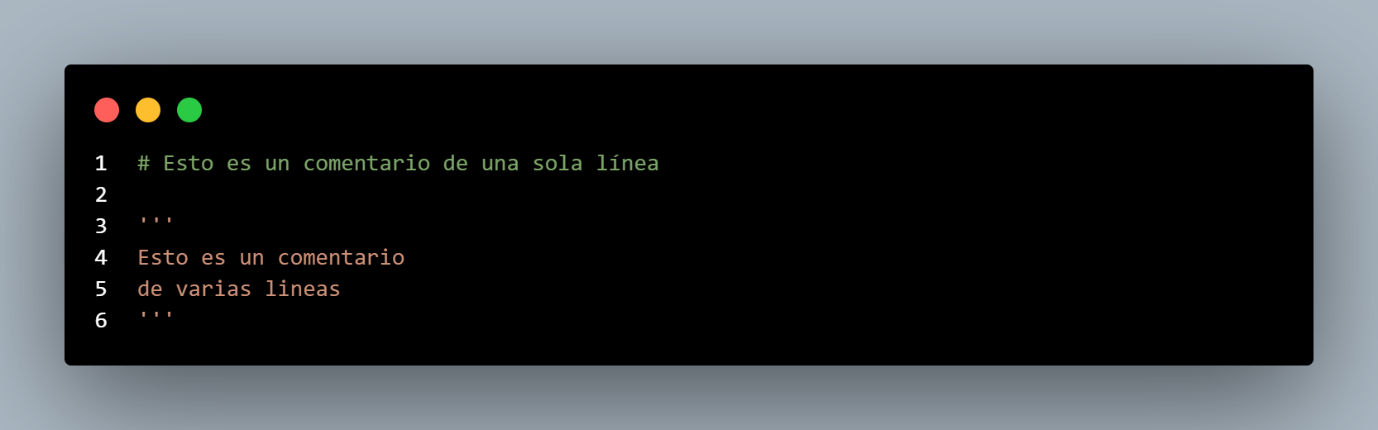
\includegraphics{Imagenes/fundamentos13.png}
    }
  \end{figure}
\begin{itemize}
    \item Comentarios de una sola línea: Se utilizan para incluir explicaciones breves en una línea.
    \item Comentarios de varias líneas: Se utilizan para describir secciones de código más largas y pueden abarcar varias líneas.
\end{itemize}

Formato de Código: El formato del código es importante para mantener la legibilidad y la consistencia en un proyecto. Python se destaca por su énfasis en la indentación (espacios al principio de una línea) para delimitar bloques de código. 
\begin{itemize}
    \item Indentación: La sangría en Python es fundamental para definir bloques de código. A diferencia de otros lenguajes que utilizan llaves o paréntesis para delimitar bloques, en Python, la sangría se utiliza para indicar la estructura del programa. Esto fomenta la legibilidad y la claridad del código. Un bloque de código se define mediante el uso de espacios o tabulaciones con un mismo nivel de sangría. 
\begin{figure}[h]
    \centering
    \scalebox{0.35}{
    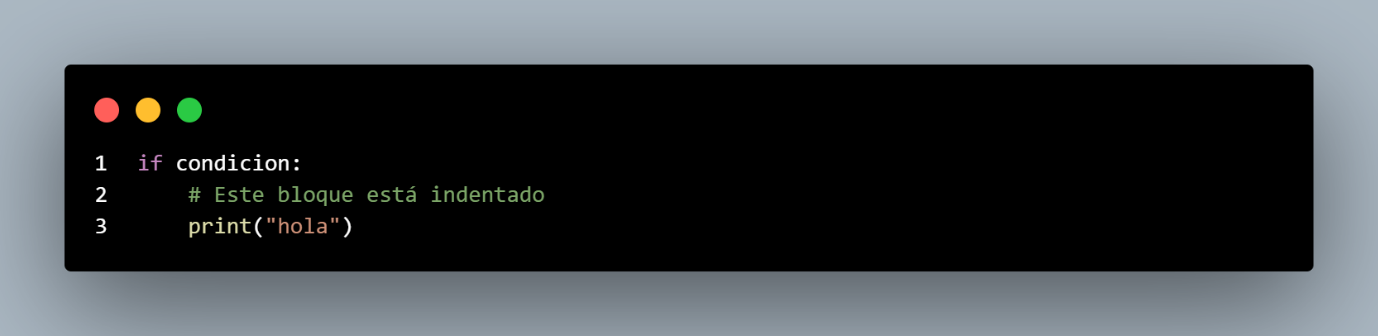
\includegraphics{Imagenes/fundamentos14.png}
    }
    \end{figure}
    \item Interpretado: Python es un lenguaje de programación interpretado. Esto significa que no es necesario compilar el código fuente en código de máquina antes de ejecutarlo. En cambio, el intérprete de Python lee y ejecuta el código línea por línea en tiempo real. Esto facilita la depuración y la portabilidad, ya que un programa escrito en Python se puede ejecutar en cualquier sistema que tenga un intérprete de Python instalado.
  \begin{figure}[h]
      \centering
      \scalebox{0.35}{
      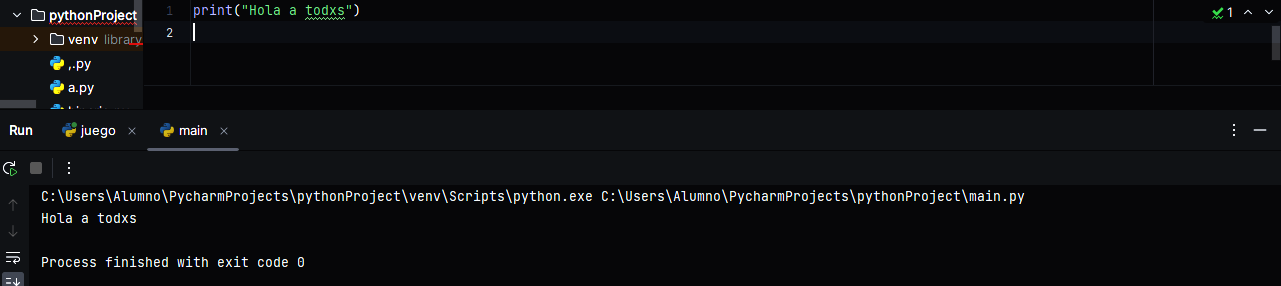
\includegraphics{Imagenes/fundamentos15.png}
      }
      \end{figure}
    \item Tipado dinámico: Python es un lenguaje de tipado dinámico, lo que significa que no necesitas declarar explícitamente el tipo de una variable al crearla. El tipo de una variable se determina automáticamente en el tiempo de ejecución según el valor que contiene. Esto permite una mayor flexibilidad, pero también significa que debes tener cuidado con los tipos de datos para evitar errores inesperados. 
\begin{figure}[h]
    \centering
    \scalebox{0.35}{
    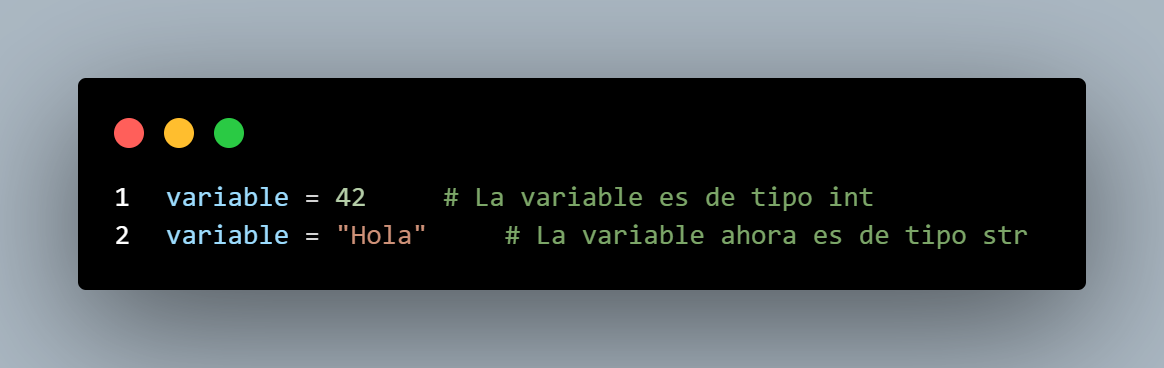
\includegraphics{Imagenes/fundamentos16.png}
    }
    \end{figure}
    \item Convenciones de Nombres: En Python, se siguen ciertas convenciones para nombrar variables, funciones y clases. Algunas pautas comunes incluyen:

\begin{itemize}
    \item Los operadores y las expresiones son componentes esenciales en Python y en la programación en general. Los operadores se utilizan para realizar operaciones en variables y valores, mientras que las expresiones son combinaciones de variables, valores y operadores que se evalúan para producir un resultado. 
    \item Variables y funciones: Usar letras minúsculas y guiones bajos para separar palabras (ejemplo: mi\_variable, mi\_funcion).
    \item Clases: Usar CamelCase (iniciar cada palabra con mayúscula, sin espacios ni guiones bajos) (ejemplo: MiClase).
    \item Constantes:Los nombres de las constantes deben estar en mayúsculas. Si es necesario separar palabras en el nombre de la constante, se pueden usar guiones bajos. Por ejemplo, PI o TASA\_DE\_INTERES.
    \item Convenciones especificas: Para indicar que una variable o función es ``privada'' (es decir, no debería accederse desde fuera de su módulo), se puede anteponer un guion bajo al nombre, por ejemplo, \_variable\_privada. Para variables que actúan como constantes y no deberían modificarse, se puede utilizar un guion bajo en mayúsculas al principio del nombre, como \_CONSTANTE.
    \item Variables temporales: En bucles y expresiones cortas, es común usar nombres de variables temporales cortos como i, j, k para iteradores. Sin embargo, es importante que estos nombres sean descriptivos dentro del contexto.
\end{itemize}

    \item Espaciado: Agregar espacios alrededor de operadores y después de comas para mejorar la legibilidad.
\newpage
    \begin{figure}[h]
        \centering
        \scalebox{0.35}{
        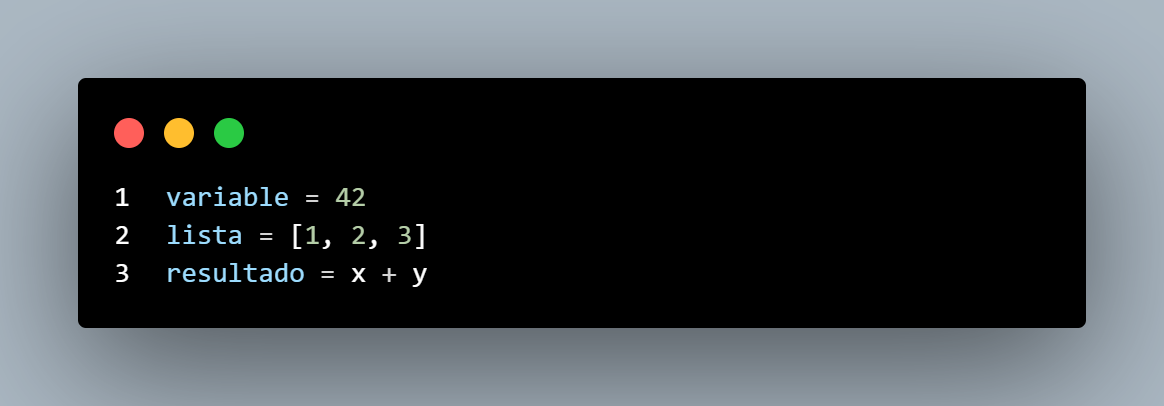
\includegraphics{Imagenes/fundamentos17.png}
        }
      \end{figure}
    \item Longitud de Línea: Es una buena práctica limitar la longitud de una línea de código a aproximadamente 79-80 caracteres para facilitar la lectura. Puedes usar una barra invertida \ para dividir una línea larga en varias líneas:
    \begin{figure}[h]
        \centering
        \scalebox{0.35}{
        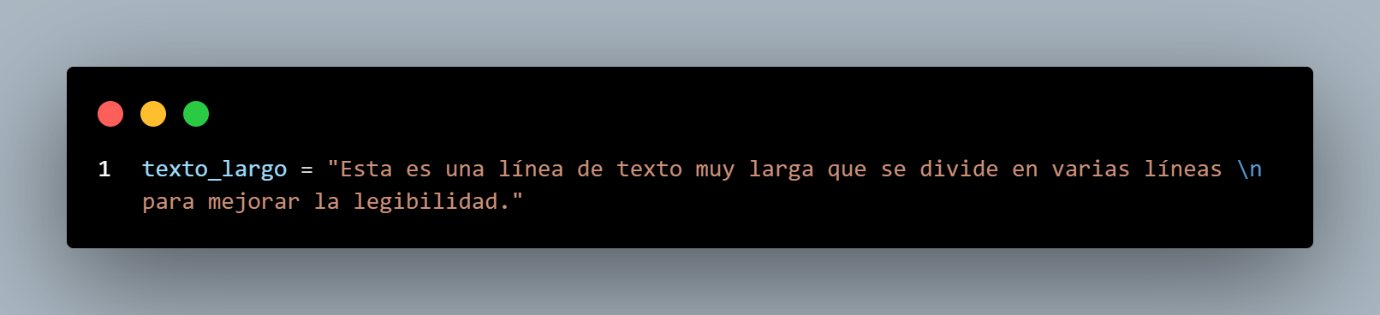
\includegraphics{Imagenes/fundamentos18.png}
        }
      \end{figure}
    \item Comentarios Descriptivos: Los comentarios deben ser informativos y explicar el propósito de una sección de código. Es especialmente útil para documentar partes complicadas o algoritmos. No es necesario comentar lo obvio.
\end{itemize}

El formato de código y los comentarios son esenciales para que tu código sea comprensible, colaborativo y mantenible. Adherirse a las convenciones de estilo y escribir comentarios informativos ayuda a otros programadores (y a ti mismo) a entender y mantener el código de manera más eficaz.


\section{Variables y tipos de datos}

\subsection{Tipos numéricos}
\subsection{Tipos de texto}
\subsection{Tipos de secuencia}
\subsection{Tipos de mapeo}
\subsection{Tipos booleanos}


\section{Estructuras de control}

\subsection{Declaraciones condicionales}
Las sentencias condicionales en Python permiten controlar el flujo del programa en función del valor de una expresión booleana. Una expresión booleana es una expresión que puede evaluarse como verdadera o falsa.\\

Sentencia if: se considera la más sencilla de las tres y toma decisiones basadas en sí la condición es verdadera o falsa. Si la condición es verdadera, se ejecuta el bloque de código sangrado. Si la condición es falsa, se omite la ejecución del bloque.\\

La sintaxis básica de la condición if es la siguiente:

Por ejemplo, el siguiente código imprime ``El número es mayor que 10'' si el número es mayor que 10:

En este ejemplo, la condición es que el número sea mayor que 10. El bloque de código contiene una sola instrucción, que es imprimir el mensaje ``El número es mayor que 10''.

Sentencia else (opcional): Puedes agregar un bloque de código que se ejecutará si la primera condición es falsa.

La sintaxis básica de la condición else es la siguiente:

Por ejemplo, el siguiente código imprime ``El número es menor que 10'' si el número es menor que 10:

En este ejemplo, la condición es que el número sea mayor que 10. El bloque de código principal se ejecuta si la condición es verdadera. Si la condición es falsa, se ejecuta el bloque de código alternativo.

Sentencia elif (opcional): Para verificar múltiples condiciones, puedes utilizar elif después de la declaración if. Ten en cuenta que solo se ejecutará el bloque de código correspondiente a la primera condición verdadera.\\

La sintaxis básica de la sentencia elif es la siguiente:


Por ejemplo, el siguiente código imprime ``El número es mayor que 10'' si el número es mayor que 10, ``El número es igual a 10'' si el número es igual a 10, y ``El número es menor que 10'' si el número es menor que 10:

En este ejemplo, la condición principal es que el número sea mayor que 10. Si la condición principal es verdadera, se ejecuta el bloque de código principal. Si la condición principal es falsa, se evalúa la primera condición elif. Si la primera condición elif es verdadera, se ejecuta el bloque de código alternativo. Si la primera condición elif es falsa, se evalúa la segunda condición elif, y así sucesivamente. Si ninguna de las condiciones elif es verdadera, se ejecuta el bloque de código else.

\subsection{Bucles y iteraciones}
En el contexto de la programación, los términos loops e iteraciones a menudo se utilizan indistintamente, pero hay una distinción sutil:

\begin{itemize}
    \item Iteración: La iteración se refiere al proceso de repetir una acción o un bloque de código para cada elemento de una secuencia o hasta que se cumpla una condición. La iteración no está limitada a los bucles, ya que puede ocurrir en otros contextos, como al recorrer elementos en una lista o realizar operaciones en un conjunto de datos.
    \item Loop (bucle): Un loop es una estructura de control que permite repetir un bloque de código múltiples veces. Puede ser un ciclo for o ``while'', y generalmente se utiliza cuando se conoce la cantidad de repeticiones necesarias. Un loop puede realizar iteraciones.
\end{itemize}

\subsection{Tipos de bucles en Python}
En Python, existen dos tipos de bucles:
\begin{itemize}
    \item Bucle for: El bucle for se utiliza para iterar sobre una colección de datos. La sintaxis es la siguiente: \\ Por ejemplo, el siguiente código imprime los números del 1 al 10:
    \item Bucle while: El bucle while se utiliza para iterar mientras una condición sea verdadera. La sintaxis es la siguiente:\\ Por ejemplo, el siguiente código imprime los números del 1 al 10:
\end{itemize}

\section{Listas, tuplas y diccionarios}

\subsection{Listas y operaciones comunes}
Las listas en python son un conjunto ordenado y editable de elementos, son dinámicas esto quiere decir que puede contener diferente tipos de datos, y aparte cabe recalcar que puede tener elementos duplicados y no generará error. Estas se pueden ocupar tanto como para recopilar datos como para organizar y alguna de sus funciones son las siguientes:

\begin{itemize}
    \item Creación de listas: Se puede crear una listas abriendo corchetes ``[]'' y separando los datos por comas ``,''
    \begin{figure}[h]
        \centering
        \scalebox{0.35}{
        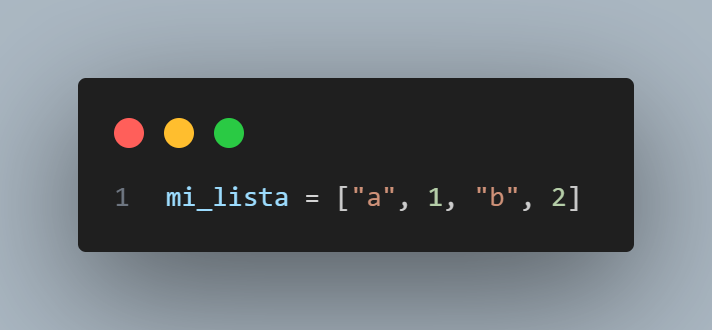
\includegraphics{Imagenes/listas1.png}
        }
      \end{figure}
    \newpage
    \item Acceso a elementos: se puede acceder a un elemento en específico de la lista poniendo el nombre de este y dentro de corchetes el número en el lugar que se encuentra  (se empieza a contar desde el 0, y para seleccionar el último será -1).
    \begin{figure}[h]
        \centering
        \scalebox{0.35}{
        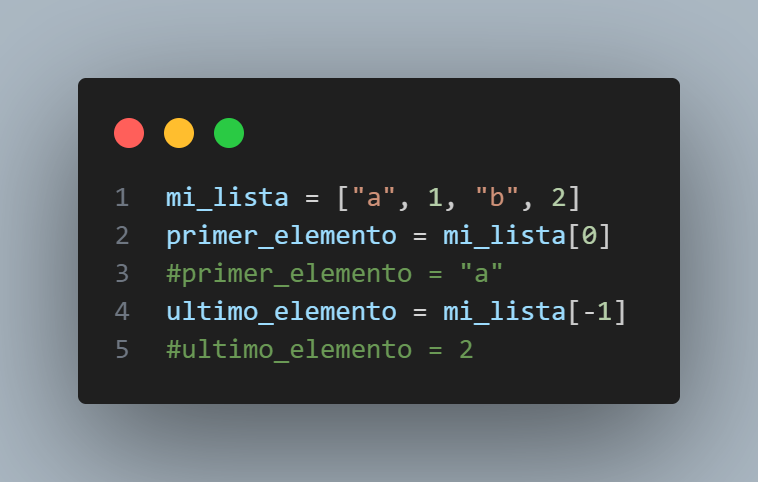
\includegraphics{Imagenes/listas2.png}
        }
      \end{figure}
    
    \item Modificar elementos: Seleccionando el puesto en el que se encuentra el dato e igualarlo al valor que queramos.
    \begin{figure}[h]
        \centering
        \scalebox{0.35}{
        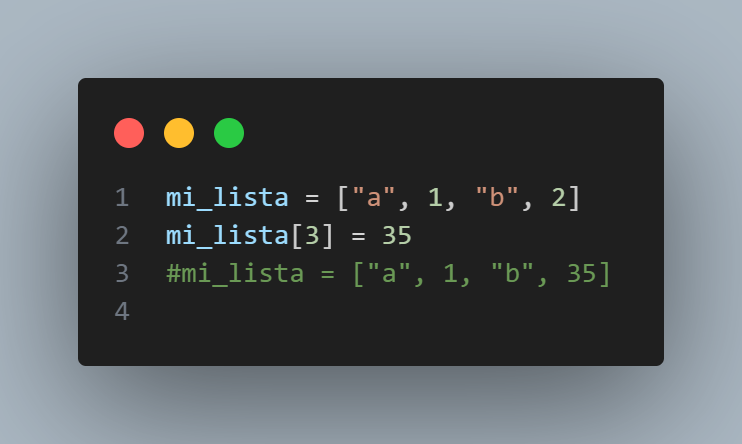
\includegraphics{Imagenes/listas3.png}
        }
      \end{figure}
    \newpage
    \item Añadir elementos: Utilizando el método ``.append(elemento)'' se pueden agregar datos.
    \begin{figure}[h]
        \centering
        \scalebox{0.35}{
        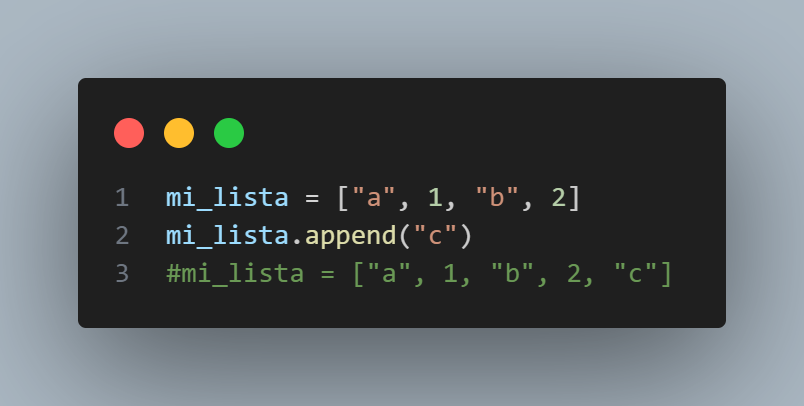
\includegraphics{Imagenes/listas4.png}
        }
      \end{figure}
    
    \item Insertar elementos: Si bien cumple la misma función que se describió anteriormente se ocupa el método ``.insert(posición, elemento)'' con esta también se puede detallar la posición en que queremos que esté.
    \begin{figure}[h]
        \centering
        \scalebox{0.35}{
        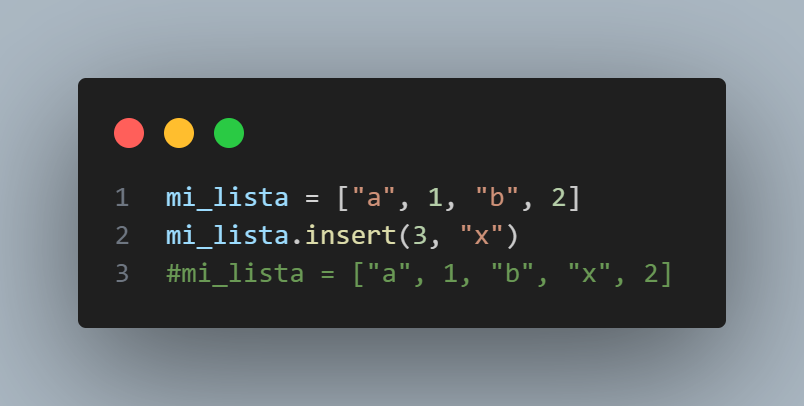
\includegraphics{Imagenes/listas5.png}
        }
      \end{figure}
    
    \item Eliminar elementos: Para eliminar elementos hay dos métodos el ``.pop(lugar del elemento)'' que elimina el dato que haya en ese puesto y el ``.remove(elemento)'' que elimina el elemento que se mencionó en los paréntesis.
    \begin{figure}[h]
        \centering
        \scalebox{0.35}{
        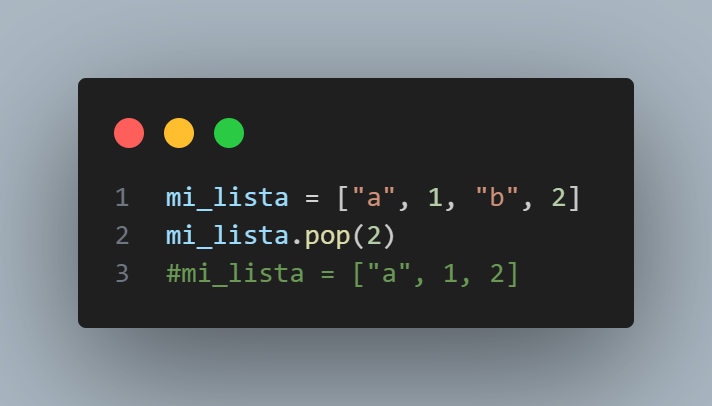
\includegraphics{Imagenes/listas6.png}
        }
      \end{figure}
    
      \begin{figure}[h]
        \centering
        \scalebox{0.35}{
        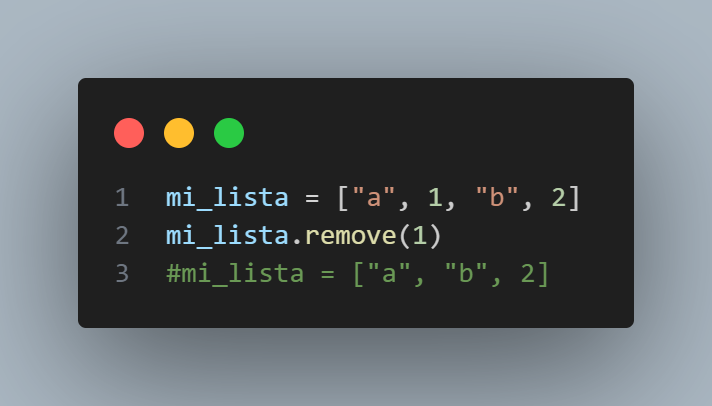
\includegraphics{Imagenes/listas7.png}
        }
      \end{figure}
\newpage
    \item Largo de una lista: Para saber cuántos elementos hay en la lista ocupamos el método ``.len(mi\_lista)''.
    \begin{figure}[h]
        \centering
        \scalebox{0.35}{
        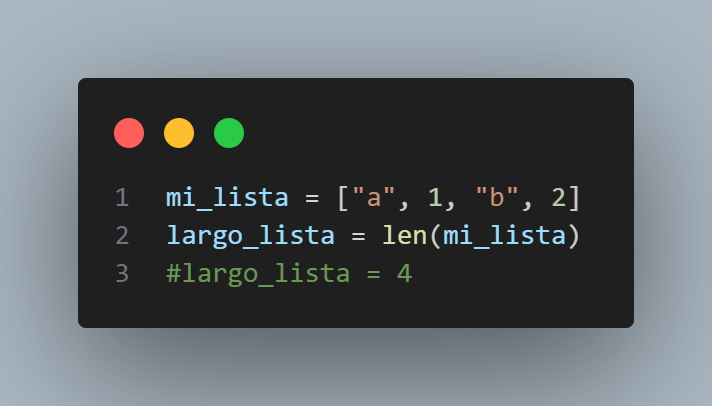
\includegraphics{Imagenes/listas8.png}
        }
      \end{figure}
    
    \item Rebanado(slicing): Puedes acceder a una porción de una lista utilizando el operador de rebanado ``[:]''.
    \begin{figure}[h]
        \centering
        \scalebox{0.35}{
        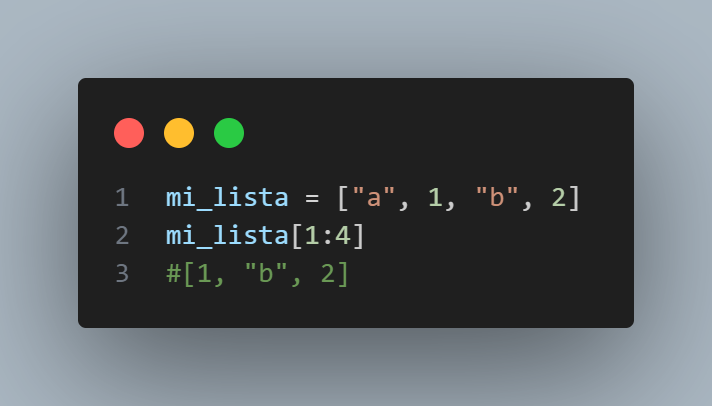
\includegraphics{Imagenes/listas9.png}
        }
      \end{figure}
    \newpage
    \item Concatenación de listas: Se pueden unir dos o más listas utilizando el operador de concatenación ``+''. 
    \begin{figure}[h]
        \centering
        \scalebox{0.35}{
        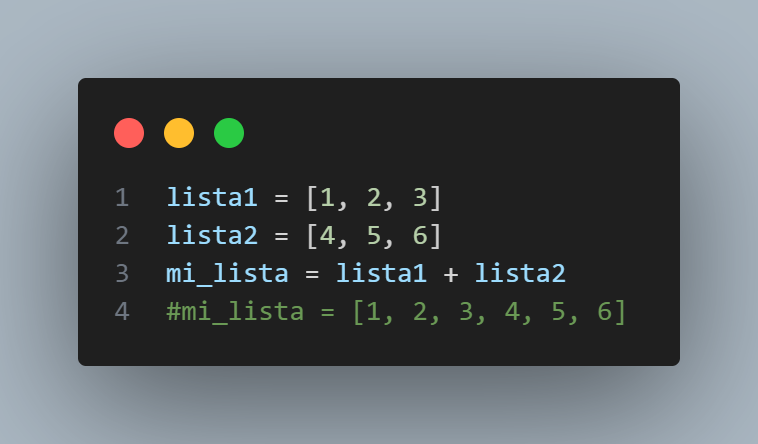
\includegraphics{Imagenes/listas10.png}
        }
      \end{figure}
    
    \item Ordenar una lista: Para ordenar una lista de manera ascendente o descendente se pueden utilizar los métodos ``.sort()'' o ``.sorted()'' respectivamente.
    \begin{figure}[h]
        \centering
        \scalebox{0.35}{
        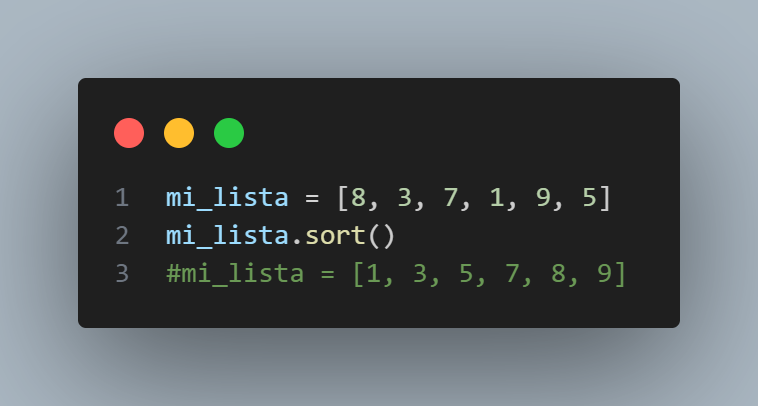
\includegraphics{Imagenes/listas11.png}
        }
      \end{figure}

      \begin{figure}[h]
        \centering
        \scalebox{0.35}{
        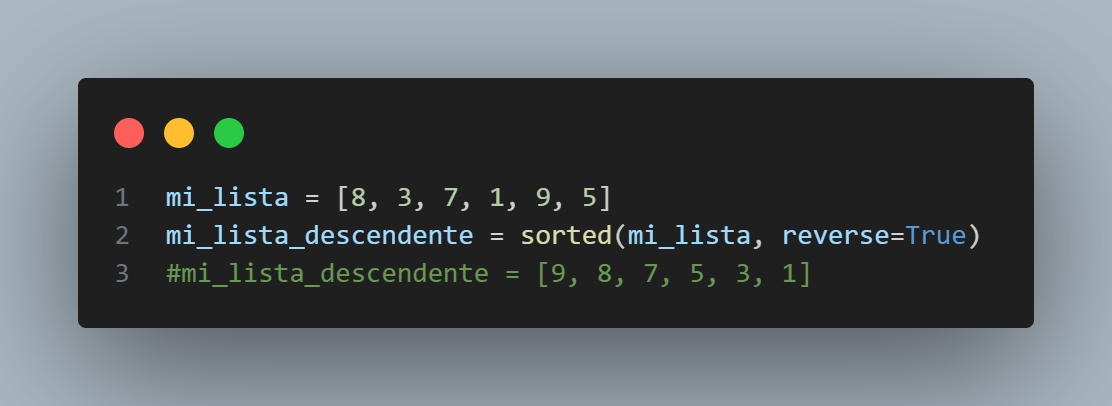
\includegraphics{Imagenes/listas12.png}
        }
      \end{figure}
    \newpage
    \item Buscar elementos:Se puede buscar un elemento de la lista utilizando el operador “in” o el método ``.index(elemento)''.
    \begin{figure}[h]
        \centering
        \scalebox{0.35}{
        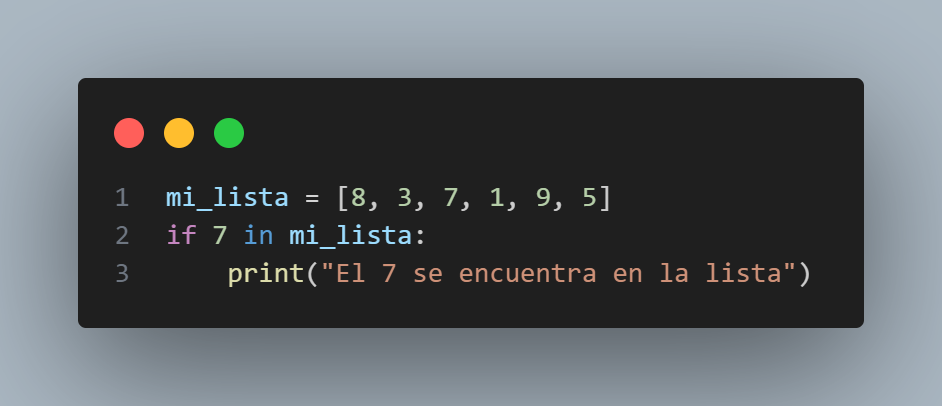
\includegraphics{Imagenes/listas13.png}
        }
      \end{figure}
    
      \begin{figure}[h]
        \centering
        \scalebox{0.35}{
        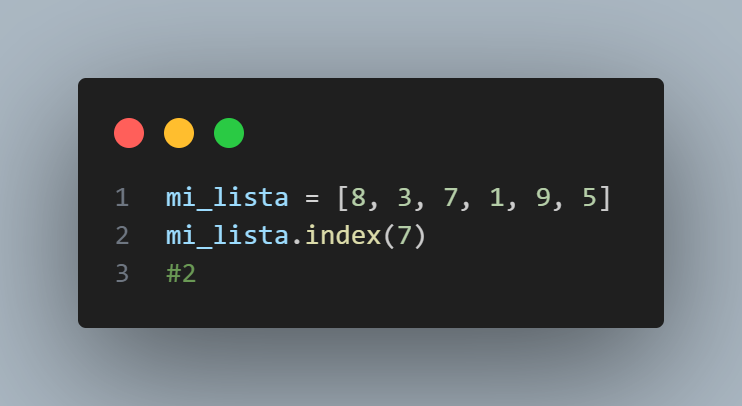
\includegraphics{Imagenes/listas14.png}
        }
      \end{figure}
\end{itemize}

\subsection{Tuplas y sus propiedades}
Si bien las tuplas son un conjunto de datos similares a las listas estas son inmutables esto quiere decir que una vez creada no se puede volver a modificar, algunas de sus propiedades son:

\begin{itemize}
    \item Creación de tuplas: Primero que nada para crear una tupla solo se necesita de paréntesis ``()'' y separar los datos por comas ``,'', aunque también se pueden crear solo separando los elementos con comas.
    \begin{figure}[h]
        \centering
        \scalebox{0.35}{
        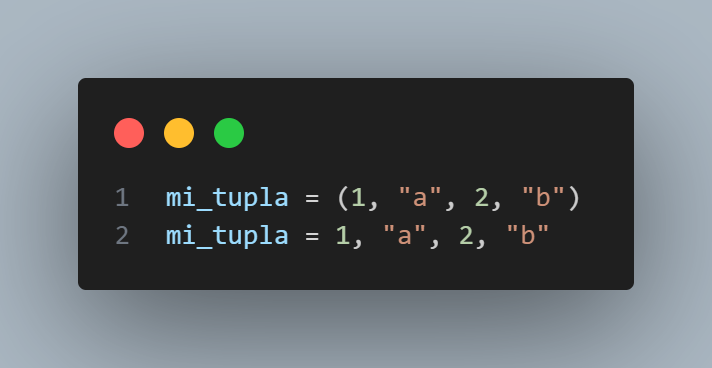
\includegraphics{Imagenes/listas15.png}
        }
      \end{figure}

    \item Acceso a elementos: Al igual que en las listas para acceder a un elemento en especifico solo se necesita de corchetes ``[índice]''.
    \begin{figure}[h]
        \centering
        \scalebox{0.35}{
        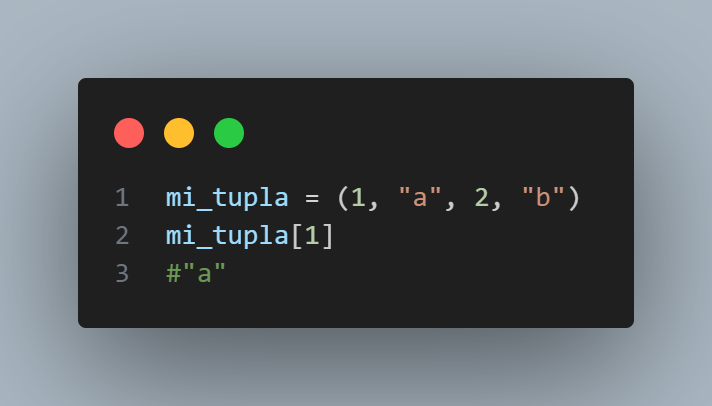
\includegraphics{Imagenes/listas16.png}
        }
      \end{figure}
    
    \item Datos inmutables: Como dije anteriormente los datos no se pueden cambiar por lo que si seleccionamos un elemento y lo tratamos de igualar a otro nos tirara un error.
    \begin{figure}[h]
        \centering
        \scalebox{0.35}{
        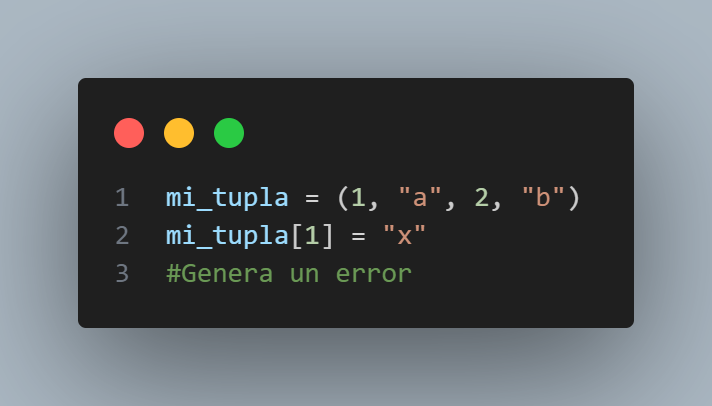
\includegraphics{Imagenes/listas17.png}
        }
      \end{figure}
    
    \item Largo de una tupla: Para saber el largo de la tupla tenemos que utilizar la función ``len(tupla)''.
    \begin{figure}[h]
        \centering
        \scalebox{0.35}{
        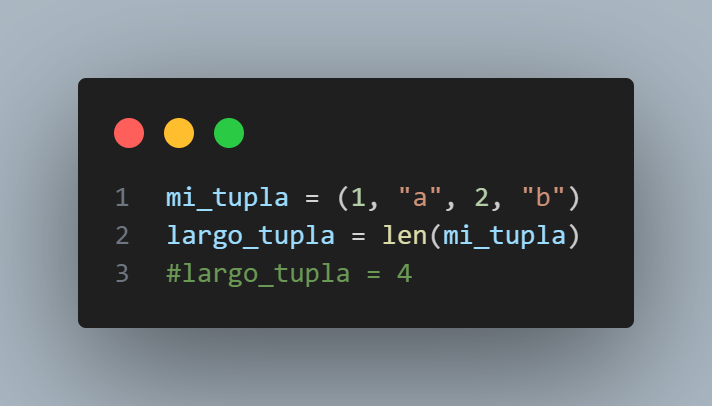
\includegraphics{Imagenes/listas18.png}
        }
      \end{figure}
    
      \newpage
    \item Rebanado (slicing): Esta propiedad sirve para seleccionar una porción de la tupla creando una nueva con estos datos y para esto necesitamos utilizar el operador de rebanado ``[:]''.
    \begin{figure}[h]
        \centering
        \scalebox{0.35}{
        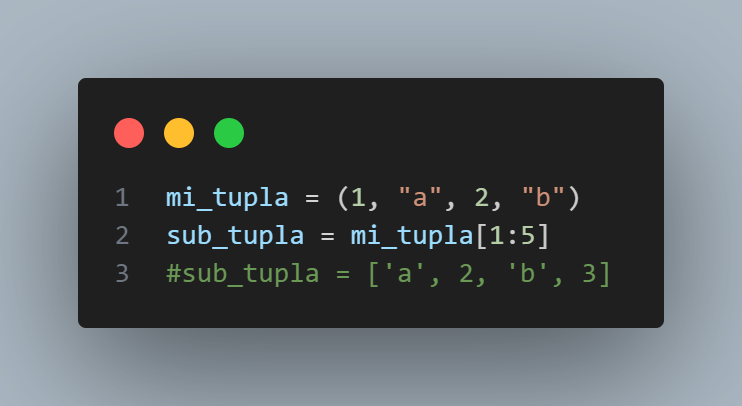
\includegraphics{Imagenes/listas19.png}
        }
      \end{figure}
    
    \item Concatenación de tuplas: Del mismo modo que en las listas para concatenar las tuplas se necesita del operador de concatenación ``+''.
    \begin{figure}[h]
        \centering
        \scalebox{0.35}{
        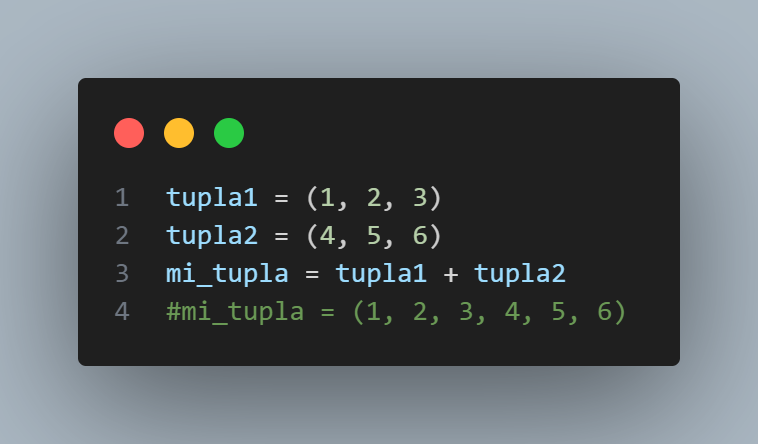
\includegraphics{Imagenes/listas20.png}
        }
      \end{figure}
    
    \item Asignación de múltiple: Este quiere decir que en una sola línea de código se puede asignar a distintas variables los elementos de la tupla. 
    \begin{figure}[h]
        \centering
        \scalebox{0.35}{
        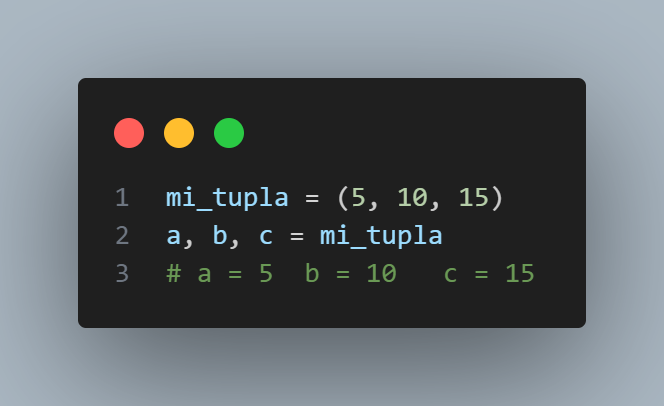
\includegraphics{Imagenes/listas21.png}
        }
      \end{figure}

\end{itemize}

\subsection{Diccionarios y métodos de acceso}
Los diccionarios en vez de las tuplas y listas contienen pares de datos que se identifican como clave-valor cada clave dentro del diccionario tiene un único valor, esto sirve para organizar todo de mejor manera y acceder a los valores de una forma mas rápida como por ejemplo:

\begin{itemize}
    \item Creación de diccionarios: Primero que nada para crear un diccionario necesitamos utilizar llaves ``{}'' y dentro separando clave-valor por ``:'' y cada par por ``,''.
    \begin{figure}[h]
        \centering
        \scalebox{0.35}{
        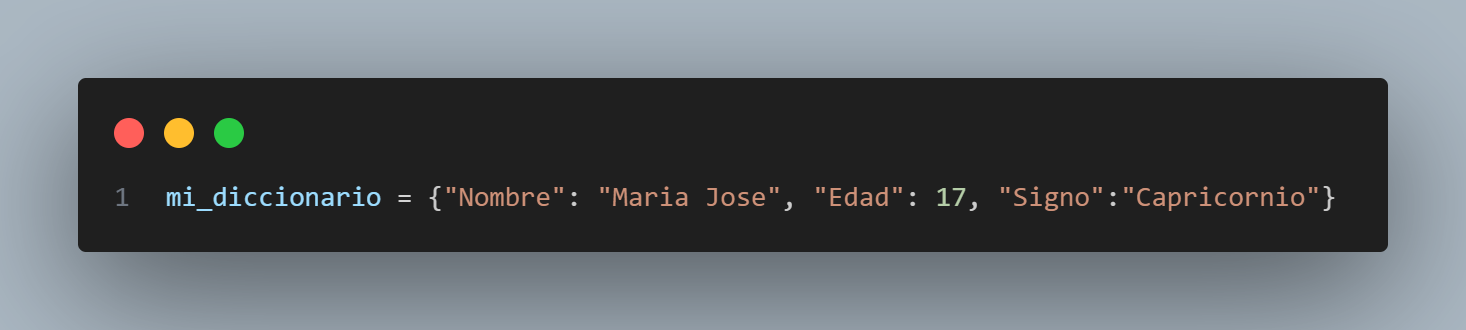
\includegraphics{Imagenes/listas22.png}
        }
      \end{figure}
    
    \item Acceso al valor: Esta vez al igual que en las anteriores se ocupan corchetes ``[clave]'' pero en vez de poner un índice esta vez se pone la clave para obtener su respectivo valor.
    \begin{figure}[h]
        \centering
        \scalebox{0.35}{
        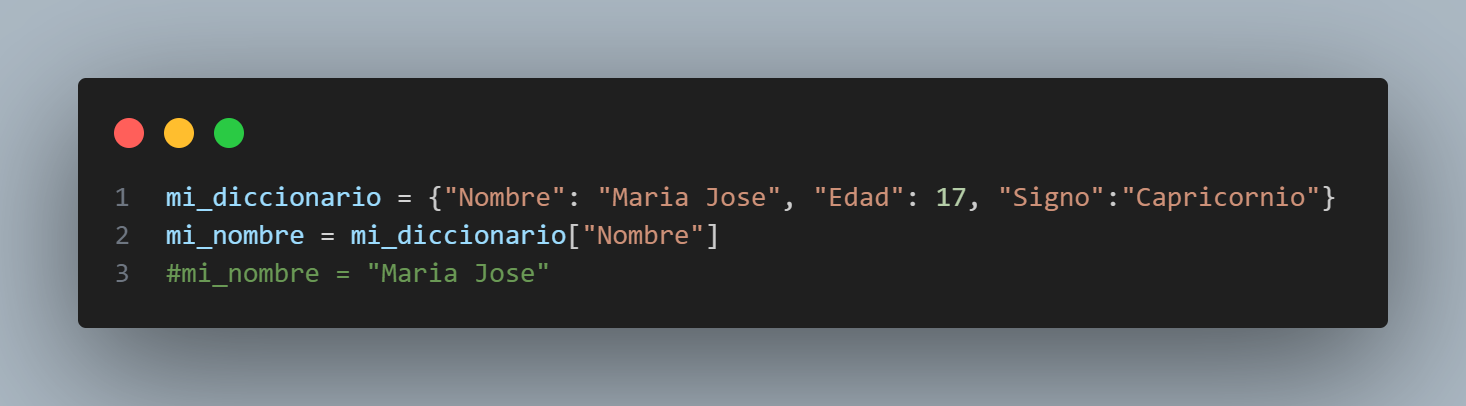
\includegraphics{Imagenes/listas23.png}
        }
      \end{figure}
    
    \item Modificación del valor: Para modificar un valor solo necesitamos seleccionar su clave e igualarlo al nuevo valor que queremos que obtenga.
    \begin{figure}[h]
        \centering
        \scalebox{0.35}{
        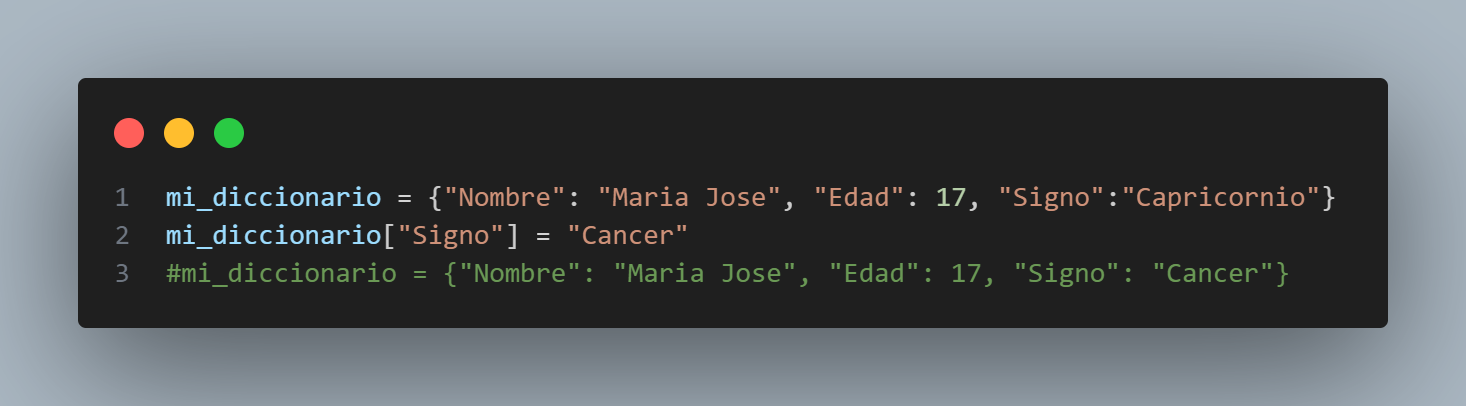
\includegraphics{Imagenes/listas24.png}
        }
      \end{figure}
    
    \item Agregar pares: Si queremos agregar nuevos pares de clave-valor solo necesitamos seleccionar una nueva clave del diccionario e igualarlo a un nuevo valor.
    \begin{figure}[h]
        \centering
        \scalebox{0.30}{
        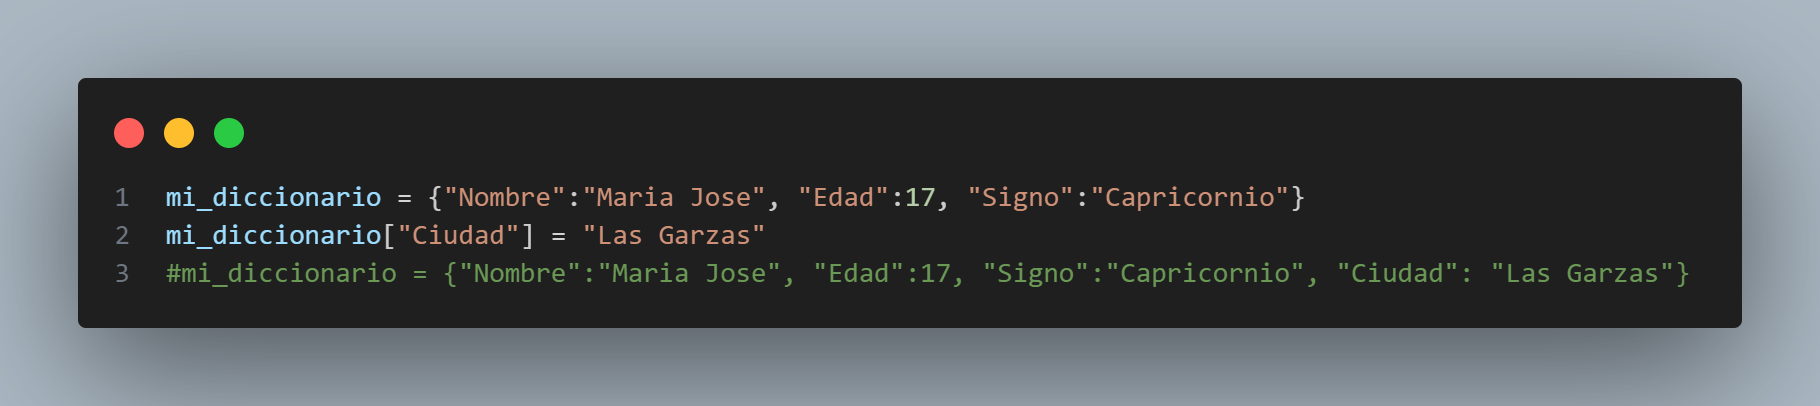
\includegraphics{Imagenes/listas25.png}
        }
      \end{figure}
    
    \item Eliminación de pares: Cuando queramos eliminar un par que este en el diccionario solo debemos utilizar la declaración ``del'' y especificar la clave.
    \begin{figure}[h]
        \centering
        \scalebox{0.35}{
        \includegraphics{Imagenes/listas26.png}
        }
      \end{figure}
    
    \item Verificación de existencia de clave: Para verificar si una clave en específico existe dentro de un diccionario podemos utilizar el operador ``in''.
    \begin{figure}[h]
        \centering
        \scalebox{0.35}{
        \includegraphics{Imagenes/listas27.png}
        }
      \end{figure}
    
    \item  Obtener clave-valor: Para obtener o todas las claves o todos los valores de un diccionario podemos utilizar los métodos ``.keys()'' o ``.values()'' respectivamente, pero si queremos obtener el par de elementos utilizaremos el método ``.items()''.
    \begin{figure}[h]
        \centering
        \scalebox{0.35}{
        \includegraphics{Imagenes/listas28.png}
        }
      \end{figure}

\end{itemize}

\section{Funciones y modularidad}


Las funciones son bloques de código reutilizables que realizan una tarea específica. Permiten dividir un programa en partes más pequeñas y manejables, lo que facilita la comprensión y el mantenimiento del código. La modularidad se refiere a la práctica de dividir un programa en módulos o funciones independientes que pueden ser desarrolladas y probadas de forma separada. Esto promueve el código limpio y organizado, facilitando la colaboración en equipos de desarrollo.

\subsection{Definición y llamada de funciones}

Definición de Funciones:\\
  
En la mayoría de los lenguajes de programación, las funciones se definen con la palabra clave ``def'' (en Python), ``function'' (en JavaScript), ``fun'' (en Kotlin), o ``void'' (en C++), seguido del nombre de la función y una lista de parámetros entre paréntesis. Por ejemplo, en Python:
\begin{figure}[h]
    \centering
    \scalebox{0.35}{
    \includegraphics{Imagenes/funciones1.png}
    }
  \end{figure}

  \newpage

Llamada de Funciones:\\

Para utilizar una función, se realiza una llamada a la función, pasando los valores necesarios como argumentos. Los argumentos son los valores reales que se pasan a la función durante la llamada. Por ejemplo:

\begin{figure}[h]
    \centering
    \scalebox{0.35}{
    \includegraphics{Imagenes/funciones2.png}
    }
  \end{figure}

En este caso, ``Juan'' es el argumento que se pasa a la función ``saludar''.

\subsection{Argumentos y parámetros}
Parámetros de Funciones:\\

Los parámetros son variables que se utilizan en la definición de la función para aceptar valores. En el ejemplo anterior, ``nombre'' es un parámetro de la función ``saludar''.
\begin{figure}[h]
    \centering
    \scalebox{0.35}{
    \includegraphics{Imagenes/funciones3.png}
    }
  \end{figure}

Argumentos de Funciones:\\

Los argumentos son los valores reales que se pasan a la función durante su llamada. En el ejemplo de la llamada a la función `saludar("Juan")`, "Juan" es el argumento que se pasa al parámetro ``nombre'' de la función ``saludar''\\

Las funciones pueden tener múltiples parámetros y se pueden pasar argumentos de diferentes tipos (números, cadenas, listas, etc.). Por ejemplo:

\newpage

\begin{figure}[h]
    \centering
    \scalebox{0.35}{
    \includegraphics{Imagenes/funciones4.png}
    }
  \end{figure}

En este caso, la función ``sumar'' tiene dos parámetros ``a'' y ``b'', y se llama con los argumentos 3 y 5, respectivamente. El resultado de la suma se almacena en la variable ``resultado\_suma''.\\

Las funciones y la modularidad son conceptos fundamentales en programación, ya que permiten escribir código más eficiente, fácil de entender y mantener. La práctica constante con estos conceptos te ayudará a mejorar tus habilidades de programación.

\subsection{Módulos y su importación}
Los módulos son archivos que contienen definiciones y declaraciones de funciones, clases y variables en Python. Ayudan a organizar el código en archivos separados para hacerlo más legible y reutilizable. Para utilizar las funciones y variables definidas en un módulo en otro archivo, se necesita importar el módulo en el archivo donde se desea utilizar.

\begin{itemize}
    \item Creación de un Módulo: Supongamos que tenemos un archivo llamado mi\_modulo.py con la siguiente definición de función:
    \begin{figure}[h]
        \centering
        \scalebox{0.35}{
        \includegraphics{Imagenes/funciones5.png}
        }
      \end{figure}
\newpage
    \item Importación de un Módulo: En otro archivo Python, podemos importar y utilizar la función saludar del módulo mi\_modulo.py de la siguiente manera:
    \begin{figure}[h]
        \centering
        \scalebox{0.35}{
        \includegraphics{Imagenes/funciones6.png}
        }
      \end{figure}
      
      También se puede importar una función específica de un módulo para evitar usar el nombre del módulo cada vez que se llama a la función:

      \begin{figure}[h]
        \centering
        \scalebox{0.35}{
        \includegraphics{Imagenes/funciones7.png}
        }
      \end{figure}
    \end{itemize}
      
    La importación de módulos es esencial para organizar proyectos grandes y complejos en Python, ya que permite dividir el código en archivos manejables y fácilmente comprensibles. Además, facilita la reutilización del código, ya que las funciones y variables definidas en un módulo pueden ser utilizadas en varios archivos del proyecto.




\section{Manejo de excepciones y errores}

\subsection{Introducción a las excepciones}
En Python, las excepciones son eventos inesperados o errores que ocurren durante la ejecución de un programa. Estos errores pueden ser causados por diversas situaciones, como divisiones por cero, acceso a archivos inexistentes o intentos de acceder a índices fuera de rango en listas. En resumen, Python nos proporciona una estructura para manejar estas excepciones y evitar que el programa se detenga abruptamente.

\subsection{Uso de try, except, else}
\begin{itemize}
    \item Try: El bloque ``try'' se utiliza para envolver el código en el que esperas que ocurra una excepción. Dentro de este bloque, colocas el código que podría generar una excepción. Si una excepción se produce en el bloque ``try'', el flujo de control se traslada al bloque ``except''.
    \item Except: El bloque ``except'' se utiliza para manejar excepciones. Puedes especificar el tipo de excepción que deseas capturar después de la palabra clave ``except''. Si ocurre una excepción del tipo especificado en el bloque try, se ejecutará el código en el bloque ``except''. Puedes tener varios bloques ``except'' para manejar diferentes tipos de excepciones.
    \begin{figure}[h]
        \centering
        \scalebox{0.35}{
        \includegraphics{Imagenes/manejo1.png}
        }
      \end{figure}
    
    
    \item Else: El bloque ``else'' es opcional y se coloca después de todos los bloques ``except''. Se ejecuta si no se ha producido ninguna excepción en el bloque ``try''. Es útil para ejecutar código que debe ejecutarse solo si no se generan excepciones.
    \begin{figure}[h]
        \centering
        \scalebox{0.35}{
        \includegraphics{Imagenes/manejo2.png}
        }
      \end{figure}
    
    \item Finally: El bloque ``finally'' es opcional y se coloca al final, después de todos los bloques ``except'' y, si se utiliza, después del bloque ``else''. El código en este bloque se ejecuta sin importar si se produjo una excepción o no. Se utiliza comúnmente para realizar la limpieza de recursos, como cerrar archivos o conexiones de bases de datos, garantizando que se realicen incluso en caso de excepciones.
    \begin{figure}[h]
        \centering
        \scalebox{0.35}{
        \includegraphics{Imagenes/manejo3.png}
        }
      \end{figure}

\end{itemize}

\subsection{Tipos de excepciones y manejo específico}
\begin{itemize}
    \item ZeroDivisionError: Se genera cuando intentas dividir un número entre cero.
    \begin{figure}[h]
        \centering
        \scalebox{0.35}{
        \includegraphics{Imagenes/manejo4.png}
        }
      \end{figure}
    \newpage
    \item FileNotFoundError: Ocurre cuando intentas abrir o realizar operaciones en un archivo que no existe.
    \begin{figure}[h]
        \centering
        \scalebox{0.35}{
        \includegraphics{Imagenes/manejo5.png}
        }
      \end{figure}
    
    \item TypeError: Esta excepción se produce cuando realizas una operación en un tipo de dato que no es compatible.
    \begin{figure}[h]
        \centering
        \scalebox{0.35}{
        \includegraphics{Imagenes/manejo6.png}
        }
      \end{figure}
    
    
    \item IndexError: Se genera al intentar acceder a un índice fuera de rango en una lista o secuencia.
    \begin{figure}[h]
        \centering
        \scalebox{0.35}{
        \includegraphics{Imagenes/manejo7.png}
        }
      \end{figure}
    
    
    \item ValueError: Esta excepción ocurre cuando el tipo de dato es correcto, pero el valor no es válido para la operación.
    \begin{figure}[h]
        \centering
        \scalebox{0.35}{
        \includegraphics{Imagenes/manejo8.png}
        }
      \end{figure}
    
    \item Custom Exceptions: Además de las excepciones incorporadas, puedes crear tus propias excepciones personalizadas extendiendo la clase Exception. Esto es útil cuando deseas manejar situaciones específicas en tu programa.
    \begin{figure}[h]
        \centering
        \scalebox{0.35}{
        \includegraphics{Imagenes/manejo9.png}
        }
      \end{figure}
    

\end{itemize}


\section{Entrada y salida de datos}

\subsection{Función print()}
La función print() en Python es una herramienta fundamental para mostrar información en la consola o en la salida estándar del programa. Su propósito principal es facilitar a lo programadores imprimir mensajes, variables, listas y otros datos que permiten observar el comportamiento del código.

\begin{itemize}
    \item Salida de texto: print() Se utiliza para mostrar cadenas de textos en la consola. Esto se útil para comunicar mensajes, indicadores o información relevante durante la ejecución del programa.
    \begin{figure}[h]
        \centering
        \scalebox{0.35}{
        \includegraphics{Imagenes/entrada1.png}
        }
      \end{figure}

    \item Imprimir variables: Imprimir variables es una práctica común en programación, ya que te permite observar el contenido de las variables en diferentes momentos de la ejecución de tu programa. Esto es esencial para el seguimiento del flujo de datos en tu código, a continuación se muestran algunos ejemplos.
\begin{itemize}
    
    \item Ejemplo 1 : Para imprimir el valor de una variable, simplemente incluye a la variable como argumento de la función.
    \begin{figure}[h]
        \centering
        \scalebox{0.35}{
        \includegraphics{Imagenes/entrada2.png}
        }
      \end{figure}

    \item Ejemplo 2 : Concatenar variables de texto. Puedes combinar el valor de una variable con texto utilizando el operador de concatenación(+). esto es útil para crear mensajes informativos
    \begin{figure}[h]
        \centering
        \scalebox{0.35}{
        \includegraphics{Imagenes/entrada3.png}
        }
      \end{figure}
\end{itemize}   
\end{itemize}

\subsection{Función input()}
Ahora cómo enviar un dato mediante el teclado para que el programa lo tome en cuenta mediante el método input()

\begin{itemize}
    \item Ejemplo 1
    \begin{figure}[h]
        \centering
        \scalebox{0.35}{
        \includegraphics{Imagenes/entrada4.png}
        }
      \end{figure}
\end{itemize}

Esta función permite obtener el texto escrito por el usuario, al cual se le asignará un espacio a la memoria con la variable que el programador crea conveniente. Al llegar a la línea del comando, la consola esperara respuesta.Cuando el usuario escriba algo y presione la tecla Enter, el código seguirá ejecutándose.\\

Lo que estamos indicando al programa es que la variable «nombre» va a tomar el valor que el usuario ingrese cuando se le muestre el mensaje «Hola ¿Cuál es tu nombre?», para posteriormente, responder con otro mensaje y el valor que se ingresó. Debemos tener en cuenta que al usar input(), los datos ingresados siempre serán guardados como tipo string. Si necesitáramos ingresar números para utilizarlos en alguna operación matemática, debemos convertirlos a un tipo de dato adecuado (por ejemplo int o float, dependiendo si requerimos decimales). Podemos hacerlo de las siguientes maneras

\begin{figure}[h]
    \centering
    \scalebox{0.35}{
    \includegraphics{Imagenes/entrada5.png}
    }
  \end{figure}

\subsection{Formateo de cadenas}

Python ofrece varias formas de formatear cadenas,y dos de los más comunes son mediantes f-strings(cadenas formateadas) y métodos de formatos.
\begin{itemize}
    \item Utilizan la sintaxis de cadenas con una “f” o “F” 
    \item Permiten incrustar expresiones o variables mediante llaves ``{}''
    \item Pueden realizar cambios y formateos dentro de la llave.
    \item Son una forma más legibles y eficiente de formatear cadenas en python.
\end{itemize}

En python, una cadena de texto normal se escribe entre comillas (``''), para crear f-strings solo tienes que agregar la letra f o F mayúscula antes de la comilla.\\

\newpage
¿Cómo imprimir variables usando f-strings?

\begin{figure}[h]
    \centering
    \scalebox{0.35}{
    \includegraphics{Imagenes/entrada6.png}
    }
  \end{figure}

¿Cómo evaluar expresiones en python con f-string?\\

Como las f-Strings son evaluadas al momento de ejecución (cuando se está ejecutando el código Python), bien podrías usar una f-string para evaluar expresiones válidas.\\

En el siguiente ejemplo. num1 y num2 son nuestras variables, para obtener el producto de estas variables únicamente basta con escribir la siguiente expresión num1 * num2 dentro de llaves
\begin{figure}[h]
    \centering
    \scalebox{0.35}{
    \includegraphics{Imagenes/entrada7.png}
    }
  \end{figure}

En cualquier f-string,  {variable nombre} y {expresión} se sustituirán  por los valores que representan  o por el valor resultante de una operación en el momento de ejecución (cuando se está ejecutando el código Python)


\section{Trabajo con archivos}

\subsection{Apertura, lectura y escritura de archivos}
Para trabajar con archivos en Python, se utiliza la función open(). Esta función toma dos argumentos: el nombre del archivo y el modo de apertura.\\

El modo de apertura determina cómo se puede acceder al archivo. Los modos de apertura más comunes son:
\begin{itemize}
    \item r: Lectura. El archivo se abre en modo de lectura.
    \item w: Escritura. El archivo se abre en modo de escritura. Si el archivo no existe, se crea uno nuevo. Si el archivo existe, se sobrescribe su contenido.
    \item a: Adición. El archivo se abre en modo de adición. Los datos se escriben al final del archivo.
\end{itemize}

Por ejemplo, para abrir un archivo de texto en modo de lectura, se puede usar el siguiente código:

Una vez que un archivo está abierto, se puede leer su contenido usando la función read(). Esta función devuelve una cadena con todo el contenido del archivo.\\

Por ejemplo, para leer el contenido de un archivo de texto, se puede usar el siguiente código:

También se puede leer el contenido de un archivo de texto línea por línea usando un bucle for:

Para escribir datos en un archivo, se usa la función write(). Esta función toma una cadena como argumento y la escribe al final del archivo.\\

Por ejemplo, para escribir el siguiente texto en un archivo de texto:

Se puede usar el siguiente código:

\subsection{Operaciones comunes de archivos}
Además de la apertura, lectura y escritura, Python ofrece otras operaciones comunes de archivos.

\begin{itemize}
    \item seek(): Permite mover el puntero de lectura o escritura a una posición determinada en el archivo.
    \item tell(): Devuelve la posición actual del puntero de lectura o escritura en el archivo.
    \item flush(): Escribe cualquier dato que aún no se haya escrito en el archivo al disco.
    \item close(): Cierra el archivo y libera los recursos asociados con él.
\end{itemize}

\subsection{Manejo de archivos con el bloque ``with''}
El bloque with es una forma segura y conveniente de abrir y cerrar archivos. Cuando se usa el bloque with, el archivo se abre automáticamente al principio del bloque y se cierra automáticamente al final del bloque.\\

Por ejemplo, el siguiente código abre un archivo de texto en modo de lectura y luego imprime su contenido:

Por ejemplo, el siguiente código abre un archivo de texto en modo de lectura y luego imprime su contenido:

El uso del bloque with evita errores comunes, como olvidar cerrar un archivo abierto.



\section{Introducción a la programación orientada a objetos}

\subsection{Definición de clases y objetos}
\subsection{Métodos y atributos de clase}

\section{Clases y objetos}

\subsection{Encapsulación y visibilidad}
\subsection{Métodos especiales}
\subsection{Herencia y composición}

\section{Herencia y polimorfismo}

\subsection{Herencia simple y múltiple}
\subsection{Polimorfismo y sobrecarga de métodos}
\subsection{Clases abstractas e interfaces}

\section{Módulos y paquetes}

\subsection{¿Qué son los Módulos en Python?}
\subsection{Creación y Uso de Módulos}
\subsection{Importación de Módulos}
\subsection{Módulos Estándar de Python}
\subsection{¿Qué son los Paquetes en Python?}
\subsection{Creación y Organización de Paquetes}
\subsection{Importación de Paquetes}

\section{Manipulación de strings y expresiones regulares}

\subsection{Operaciones comunes con cadenas de texto}
\subsection{Operaciones comunes con cadenas de texto}

\section{Trabajo con fechas y tiempos}

\subsection{Módulos datetime y time}
\subsection{Operaciones y formateo de fechas y tiempos}

\section{Introducción a Git}

\subsection{¿Qué es Git y por qué es importante?}
\subsection{Configuración inicial de Git}
\subsection{Comandos básicos de Git}

\section{Creación de interfaces gráficas con bibliotecas como Tkinter}

\subsection{Introducción a las interfaces gráficas}
\subsection{Uso de Tkinter para GUÍAs simples}


\end{document}
